\documentclass[11pt]{article}

\usepackage{extras} % Se extras.sty
\usepackage{listings}
\lstset{tabsize = 2}

\begin{document}
\begin{titlepage}
\begin{center}

{\Large\bfseries TSEA56 - Kandidatprojekt i elektronik \\ LIPS Teknisk dokumentation}

\vspace{5em}

Version 1.0

\vspace{5em}
Grupp 4 \\
\begin{tabular}{rl}
Hynén Ulfsjöö, Olle&\verb+ollul666+
\\
Wasteson, Emil&\verb+emiwa068+
\\
Tronje, Elena&\verb+eletr654+
\\
Gustafsson, Lovisa&\verb+lovgu777+
\\
Inge, Zimon&\verb+zimin415+
\\
Strömberg, Isak&\verb+isast763+
\\
\end{tabular}

\vspace{5em}
\today

\vspace{16em}
Status
\begin{longtable}{|l|l|l|} \hline

Granskad & - & - \\ \hline
Godkänd & - & - \\ \hline
 
\end{longtable}

\end{center}
\end{titlepage}

\pagebreak
\begin{center}

\section*{PROJEKTIDENTITET}
2016/VT, Undsättningsrobot Gr. 4

Linköpings tekniska högskola, ISY
\vspace{5em}
%\begin{center}

\begin{tabular}{|l|l|l|l|} \hline
\textbf{Namn} & \textbf{Ansvar} & \textbf{Telefon} & \textbf{E-post}  \\ \hline 
Isak Strömberg (IS) & Projektledare & 073-980 38 50 & isast763@student.liu.se \\ \hline
Olle Hynén Ulfsjöö (OHU)& Dokumentansvarig & 070-072 91 84 & ollul666@student.liu.se \\ \hline
Emil Wasteson (EW) & Hårdvaruansvarig & 076-836 61 66 & emiwa068@student.liu.se \\ \hline
Elena Tronje (ET) & Mjukvaruansvarig & 072-276 92 93 & eletr654@student.liu.se \\ \hline
Zimon Inge (ZI)& Testansvarig & 070-171 35 18 & zimin415@student.liu.se \\ \hline
Lovisa Gustafsson (LG) & Leveransansvarig & 070-210 32 53 & lovgu777@student.liu.se \\ \hline
\end{tabular}

%\end{center}

E-postlista för hela gruppen: isast763@student.liu.se

\vspace{5em}
Kund: ISY, Linköpings universitet 
tel: 013-28 10 00, fax: 013-13 92 82 \\
Kontaktperson hos kund: Mattias Krysander \\
tel: 013-28 21 98, e-post: matkr@isy.liu.se \\

\vspace{5em}
Kursansvarig:  Tomas Svensson\\
tel: 013-28 13 68, e-post: tomass@isy.liu.se \\
Handledare: Peter Johansson \\
tel: 013-28 13 45, e-post: peter.a.johansson@liu.se
\end{center}
\pagebreak

\tableofcontents

\pagebreak

\section*{Dokumenthistorik}
\begin{table}[h]
\begin{tabular}{|l|l|l|l|l|} \hline

\textbf{Version} & \textbf{Datum} & \textbf{Utförda förändringar} & \textbf{Utförda av} & \textbf{Granskad} \\ \hline
1.0 & - &  Första utkastet & Grupp 4 & - \\ \hline
\end{tabular}
\end{table}

\pagebreak
\pagenumbering{arabic}

\begin{flushleft}
\section{Inledning}

Projektets syfte är att konstruera en undsättningsrobot med kartläggning. Detta dokument syftar till att ge en detaljerad teknisk beskrivning av projektet. Innehållet består av beskrivningar av systemets olika delar, dess mjuk- och hårdvarukomponenter samt hur dessa är implementerade.

\section{Produkten}
Produkten som konstruerats är en undsättningsrobot. Den består av ett chassi inklusive ett batteri, en av/på-brytare samt en gripklo. På chassit är huvudmodulen, sensormodulen och styrmodulen ihopkopplade med en I\textsuperscript{2}C-buss som sköter kommunikationen mellan dem. Roboten kommunicerar med datormodulen via Bluetooth\textsuperscript{\circledR}. Gripklon kontrolleras av styrmodulen och  det är sensormodulen som tar in data från sensorerna. För att montera sensorerna på chassit har fästen utskrivna med 3D-skrivare använts. En översiktlig bild av produkten återfinns i figur \ref{overview}.

Varje modul har en processor och övrig nödvändig hårdvara, som lågpassfilter och brytare, kopplade på ett virkort. Virkorten kan användas som grund för att tillverka kretskort med motsvarande funktion. 

Robotens uppgift är att söka av en labyrint och identifiera en nödställd som sänder ut IR-ljus. När målet är identifierat bestäms kortaste vägen mellan labyrintens ingång och målet. Efter det hämtar roboten en förnödenhet vid starten, kör kortaste vägen till den nödställde och lämnar av förnödenheten för att sedan ta sig tillbaka samma väg till starten. Utforskning och intern kartläggning av labyrinten sker simultant. Informationen lagras för att kunna skickas vidare till datormodulen för uppritning. 


\begin{figure}[!htbp]
\centering
\noindent\resizebox{\linewidth}{!}{
	
\documentclass[border=10px]{standalone}
\usepackage{tikz}
\usetikzlibrary{patterns}
\usetikzlibrary{shapes.arrows}
\usepackage{amssymb}
\usetikzlibrary{calc}
\usepackage{verbatim}
\usetikzlibrary{decorations.pathmorphing}

\begin{document}
	
\begin{tikzpicture}[scale=1,rotate=0]
		
	%Base
	\draw[thick, draw=black, fill=gray!10] (0,0) rectangle (6,10);

	%Wheels
	\draw[thick, pattern=north west lines, pattern color=black] (-.5,1) 		rectangle (0,2.5);
	\draw[thick, pattern=north west lines, pattern color=black] (-.5,7.5) 	rectangle (0,9);
	\draw[thick, pattern=north west lines, pattern color=black] (6,1) 		rectangle (6.5,2.5);
	\draw[thick, pattern=north west lines, pattern color=black] (6,7.5) 		rectangle (6.5,9);
	
	%Sensors
	\draw[thick, draw=black, fill=white]		(-.25,.25) 		rectangle 	(.5,.75);
	\draw[thick, draw=black, fill=white] 	(-.25,9.25) 		rectangle 	(.5,9.75);
	\draw[thick, draw=black, fill=white] 	(5.5,.25) 		rectangle 	(6.25,.75);
	\draw[thick, draw=black, fill=white] 	(5.5,9.25) 		rectangle 	(6.25,9.75);
	\draw[thick, draw=black, fill=white] 	(1.5,10.25) 		rectangle 	(4.5,9.5);
	\draw[thick, draw=black]				 	(2.5,9.5)			--		  	(2.5,10.25);
	\draw[thick, draw=black]					(3.5,9.5) --++ (0,.75);
	
	%Gripklo
	\draw[thick, draw=black, <-] (3,10.25) --++ (0,.72) node[above] {Gripklo};
	
	%Lidar lite
	\draw[thick, draw=black, <-] 			(1.5,10.25)  		--+ 		  	(135:1) node[above, align=center] {\verb+LIDAR-Lite v2+ \\ med servo};
	%Identifierare av nödställd
	\draw[thick, draw=black, <-]				(4.5,10.25)		--+			(45:1)  node[above] {\verb+IRM-8601-S+};
	
	%IR sensorer
	\draw[thick, draw=black, <-]				(-.25, 9.75) 	--+			(135:1) node[above] {\verb+GP2D120+};
	\draw[thick, draw=black, <-]				(-.25, .25) 		--+			(225:1) node[below] {\verb+GP2D120+};
	\draw[thick, draw=black, <-]				(6.25, 9.75) 	--+			(45:1) node[above] {\verb+GP2D120+};
	\draw[thick, draw=black, <-]				(6.25, .25) 		--+			(315:1) node[below] {\verb+GP2D120+};
	
	\draw[thick, draw=black, fill=white]					(2.5,4.5)		rectangle	(3.5,5.5);
	
	%Gyro
	\draw[thick, draw=black, <-] (3.5,5) --++ (.25,0) node[rotate=270, above] {\verb+MLX90609+};
	
	%Arrows and text
	%\draw[thick, ->]  (3,11) node[left, align=center] {\verb+LIDAR-Lite v2+ \\ + detektor av nödställd} -- (3,10.25);
	%\draw[thick, <->] (0.5,0.5)  --  (5.5,0.5) node[left=-14pt,midway, fill=gray!10] {\verb+GP2D120+};
	%\draw[thick, <->] (0.5,9.5) -- (3,9) node[right=-14pt,fill=gray!10] {\verb+GP2D120+} -- (5.5,9.5);
	%\draw[thick, ->] (4.5,5) node[above] {\verb+MPU-6500+} -- (3.5,5);
	
	%Sensormodul
	\node (sensormodul) at (3,6.75) [thick, draw=black, minimum width=3cm, minimum height=1.5cm, align=center, fill=white] {Sensormodul \\ \verb+ATmega1284p+};
	
	%Huvudmodul
	\node (huvudmodul) at (3,3.25) [thick, draw=black, minimum width=3cm, minimum height=1.5cm, align=center, fill=white] {Huvudmodul \\ \verb+ATmega1284p+};
	
	%Styrmodul
	\node (styrmodul) at (3,1.25) [thick, draw=black, minimum width=3cm, minimum height=1.5cm, align=center, fill=white] {Styrmodul \\ \verb+ATmega1284p+};
	
	%I2C-buss
	\draw[thick, draw=teal] ($(sensormodul.north east) + (.25,0)$) -- ($(styrmodul.south east) + (.25,0)$);
	\draw[thick, draw=teal] ($(sensormodul.north east) + (.5,0)$) -- ($(styrmodul.south east) + (.5,0)$);
	\node (i2c) at ($(sensormodul.north east) + (0.375,.25)$) [text=teal] {\small I\textsuperscript{2}C};
	
	\draw[thick, draw=teal, fill=teal] ($(sensormodul.south east) + (0,.25)$) --+ (.25,0) circle [radius=.05cm];
	\draw[thick, draw=teal, fill=teal] ($(sensormodul.south east) + (0,.5)$) --+ (.5,0) circle [radius=.05cm];
	
	\draw[thick, draw=teal, fill=teal] ($(huvudmodul.south east) + (0,.25)$) --+ (.25,0) circle [radius=.05cm];
	\draw[thick, draw=teal, fill=teal] ($(huvudmodul.south east) + (0,.5)$) --+ (.5,0) circle [radius=.05cm];
	
	\draw[thick, draw=teal, fill=teal] ($(styrmodul.south east) + (0,.25)$) --+ (.25,0) circle [radius=.05cm];
	\draw[thick, draw=teal, fill=teal] ($(styrmodul.south east) + (0,.5)$) --+ (.5,0) circle [radius=.05cm];
	
	%Koppling till sensormodul
	\draw[thick, draw=violet] (.5,9.5) --++ (.25,0) --++ (0,-2.5) --++ (0.75,0) ;
	\draw[thick, draw=violet] (.5,.5) --++ (.25,0) --++ (0,6.25) --++ (0.75,0);
	
	\draw[thick, draw=violet] (5.5,9.5) --++ (-.25,0) --++ (0,-2.5) --++ (-0.75,0);
	\draw[thick, draw=violet] (5.5,.5) --++ (-.25,0) --++ (0,6.25) --++ (-0.75,0);
	
	\draw[thick, draw=violet] (2,9.5) --++ (0,-2);
	\draw[thick, draw=violet] (4,9.5) --++ (0,-2);
	
	\draw[thick, draw=violet] (sensormodul.south) --++ (0,-.5);
	
	%Kopplingar till styrmodul
	\draw[thick, draw=olive] (styrmodul.east) --++ (1.5,0);
	\draw[thick, draw=olive] (styrmodul.west) --++ (-1.5,0);
	\draw[thick, draw=olive] ($(styrmodul.east) + (0,.25)$) --++ (1,0) --++ (0,6.25) --++ (.5,0);
	\draw[thick, draw=olive] ($(styrmodul.west) + (0,.25)$) --++ (-1,0) --++ (0,6.25) --++ (-.5,0);
	\draw[thick, draw=olive] (3,9.5) --++ (0,-1.75) --++ (-1.75,0) --++ (0,-6) --++ (.25,0);
	
	%Bluetooth
	\draw[thick, draw=black] (huvudmodul.east) --++ (2,0) node[right,minimum width=.75cm, minimum height=1cm, draw=black] (bt) {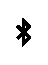
\includegraphics{bluetooth}};
	
	\node (bt2) at ($(bt) + (2,0)$) [thick, draw=black, minimum width=.75cm, minimum height=1cm] {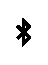
\includegraphics{bluetooth}};
	
	\draw[thick, ->,line join=round,decorate, decoration={
    												snake,
    												segment length=5,
    												amplitude=1,
    												post=lineto,
    												post length=1pt}] 
    		($(bt.east) + (5pt,5pt)$) -- ($(bt2.west) + (-5pt,5pt)$);
    		
    \draw[thick, ->,line join=round,decorate, decoration={
    												snake,
    												segment length=5,
    												amplitude=1,
    												post=lineto,
    												post length=1pt}] 
    		 ($(bt2.west) + (-5pt,-5pt)$) -- ($(bt.east) + (5pt,-5pt)$);
    		 
    \draw[thick, draw=black] (bt2.east) --++ (.5,0) node[right, minimum width=3cm, minimum height=1.5cm, draw=black, fill=white] {Datormodul};
    
    \draw[thick, draw=black] ($(sensormodul.south west) + (.25,0)$) --++ (0,-2) node[midway, above, sloped] {\small avbrott};
    
    \draw[thick, draw=black] ($(styrmodul.north west) + (.25,0)$) -- ($(huvudmodul.south west) + (.25,0)$) node[right, midway] {\small avbrott};
	
	\end{tikzpicture}
	
\end{document}  
}
	\caption{Det totala systemet \label{overview}}	
\end{figure}

\subsection{Begränsningar}
Roboten är begränsad till att navigera i korridorer och kräver att alla korsningar består av 90-gradersvinklar. Labyrinten måste bestå av moduler med storlek 40x40 centimeter.

\pagebreak

\section{Teori}
I följande avsnitt lyfts teori som är nödvändig för förståelse av implementationen.

\subsection{Labyrintnavigering}
Nedan beskrivs principer för avsökning och kartläggning av labyrinter.

\subsubsection{Väggföljare}
Ifall labyrinten är enkelt sammanhängande räcker en väggföljar-algoritm för att kartlägga alla korridorer. I en enkelt sammanhängande labyrint är alla väggar kopplade till varandra, se figur \ref{maze} för exempel. En väggföljar-algoritm är antingen av höger- eller vänstertyp och bygger på att en av korriodens sidor alltid följs. Ifall algoritmen är av högertyp följs höger sida av korridoren, vice versa för vänstertyp.

\begin{figure}[htbp]
	\centering
	\begin{subfigure}{.5\linewidth}
		\centering
		\noindent\resizebox{.5\textwidth}{!}{
			\documentclass[border=10px]{standalone}
\usepackage{tikz}
\usetikzlibrary{patterns}
\usetikzlibrary{shapes.arrows}
\usepackage{amssymb}
\usetikzlibrary{calc}
\usepackage{verbatim}
\begin{document}
	
\begin{tikzpicture}[scale=1]
		
		
		\draw[thick, ,draw=none, pattern=north west lines, pattern color=green] (1,1) rectangle (2,2);
		\draw[thick] (0,0) -- (0,4) -- (4,4) -- (4,0) -- (1,0);
		\draw[thick] (1,3) -- (1,1) -- (3,1) -- (3,3) -- (2,3);
		\draw[thick] (1,2) -- (2,2);
		
		\draw[thick, ->] (.5,-.5) -- (.5,-0);
		
		\draw[thick, ->,loosely dotted, draw=blue] (.2,0) -- (.2,3.8) -- (3.8,3.8) -- (3.8,.2) -- (1,.2);
		
	\end{tikzpicture}
\end{document}}
		\caption{En inte enkelt sammanhängande labyrint}	
		\label{non-connected}
	\end{subfigure}%
	\begin{subfigure}{.5\linewidth}
		\centering
		\noindent\resizebox{.5\textwidth}{!}{
			\documentclass[border=10px]{standalone}
\usepackage{tikz}
\usetikzlibrary{patterns}
\usetikzlibrary{shapes.arrows}
\usepackage{amssymb}
\usetikzlibrary{calc}
\usepackage{verbatim}
\begin{document}
	
\begin{tikzpicture}[scale=1]
		
		
		\draw[thick, ,draw=none, pattern=north west lines, pattern color=green] (1,1) rectangle (2,2);
		\draw[thick] (0,0) -- (0,4) -- (4,4) -- (4,0) -- (1,0);
		\draw[thick] (1,3) -- (1,1) -- (3,1) -- (3,3) -- (2,3);
		\draw[thick] (1,2) -- (2,2);
		\draw[thick] (3,1) -- (4,1);
		
		\draw[thick, ->] (.5,-.5) -- (.5,-0);
		
		\draw[thick, ->, loosely dotted, draw=blue] (.2,0) -- (.2,3.8) -- (3.8,3.8) -- (3.8,1.2) -- (3.2,1.2) -- (3.2,3.2) -- (1.8,3.2) -- (1.8,2.8) -- (2.8,2.8) -- (2.8,1.2) -- (2,1.2);
		
	\end{tikzpicture}
\end{document}}
		\caption{En enkelt sammanhängande labyrint}	
	\end{subfigure}%
	\caption{Exempel på labyrint och rutt som skulle tas av en väggföljningsalgoritm av vänstertyp}
	\label{maze}
\end{figure}%

Fördelar med algoritmen är att den är enkel att implementera men avsaknaden av intelligens gör att utforskandet av labyrinten tar lång tid. Algoritmen klarar endast att utforska de allra enklaste typer av labyrinter och ifall labyrinten inte är enkelt sammanhängande kan roboten fastna i en oändlig loop.

\subsubsection{\emph{Dead-end filling}}
\emph{Dead-end filling} är en djup-först-algoritm som utforskar en väg tills en återvändsgränd upptäcks. Därefter åker roboten tillbaka till den första korsningen som har outforskade utgångar och kartlägger dessa tills en ny återvändsgränd upptäcks. Denna process återupprepas tills hela labyrinten är kartlagd.

\subsection{Beräkning av kortaste väg}
Nedan beskrivs två algoritmer för att ta fram kortaste väg.

\subsubsection{Dijkstras algoritm}
Dijkstras algoritm är en girig, bäst-först-algoritm. Algoritmen beräknar den billigaste vägen från startnoden till samtliga noder och fungerar på nätverk med icke-negativa bågkostnader. 

Vid starten definieras två mängder, en med de avsökta och en med de oavsökta noderna. De oavsökta noderna har ett oändligt nodpris och startnoden har nodpriset noll. Med ursprung i startnoden söker algoritmen igenom alla grannar. Nodpriset uppdateras i det fall då sambandet

\begin{displaymath}
	y_i + c_{i,j} < y_j
\end{displaymath}

gäller, där \begin{math} y_i \end{math} är nodpriset för den nod som söks av, \begin{math} y_j \end{math} är nodpriset för nodgrannen och \begin{math} c_{i,j} \end{math} är kostnaden mellan nod \begin{math} i \end{math} och \begin{math} j \end{math}. Ovanstående görs successivt med ursprung i den nod med billigast nodpris som även tillhör den oavsökta mängden, tills slutnoden har undersökts. Den kortaste vägen kan sedan nästlas upp, förutsatt att den föregående noden som bidrog till den kortaste vägen sparas. 

\subsubsection{A*}
A* är ytterligare en bäst-först-algoritm med målet att finna den billigaste vägen mellan två noder. I grund och botten finns samma maskineri som i Dijkstras algoritm, med skillnaden att noder avsöks i stigande ordning enligt
\begin{equation*}
	f(n) = g(n) + h(n)
\end{equation*}
där $g(n)$ utgör kostnaden av rutten från startnod till nod $n$ och $h(n)$ en heuristik som estimerar den billigaste vägen från nod $n$ till slutnod. Med andra ord är Dijkstras algoritm ett speciallfall av A* där $h(n) = 0$.

$h(n)$ kan ses som en straffunktion som avtar nära slutnoden. A* kan alltså, till skillnad från Dijkstras algoritm, se framåt i nätverket och kan därför ta bättre beslut om vilka noder som ska uppdateras.

\subsection{Reglering}\label{subsection:reglering}
Roboten har två olika reglermoder: reglering av rotation och reglering av rak körning. Regleringen av rak körning har i sin tur fyra olika lägen: inga väggar, vägg på vänster sida, vägg på höger sida och vägg på båda sidor. Detta avgör sedan vilken insignal som används i regleringen.

Rotation regleras genom öppen reglering. Robotens gyro ger en vinkelhastighet som sedan integreras (summeras) tills summan nått ett förutbestämt värde, varefter rotationen avbryts.

Reglering av rak körning innebär reglering av två utsignaler: robotens avstånd till framförvarande vägg och robotens avstånd till väggen/väggarna i korridoren. Avståndet till framförvarande vägg $s$ regleras i förhållande till det önskade avståndet $s^0$ genom reglering av hastigheten $v$ enligt följande ekvation
\begin{equation*}
	v = 
	\begin{cases}
		v_{pref} \qquad\qquad \forall \ (s - s^0) > 20 \\
		0.6 \cdot v_{pref} \qquad \forall \ 20 \geq (s - s^0) > 0 \\
		0 \qquad\qquad\qquad \forall \ (s - s^0)\leq 0 \\
	\end{cases}
\end{equation*}
där $v_{pref}$ är den användardefinierade maxhastigheten.

Avståndet till väggen regleras genom att beräkna önskad skillnad i hastighet mellan höger och vänster hjulpar $\Delta v$ utifrån främre sidosensor $d_1$, bakre sidosensorn $d_2$ och det önskade avståndet $d^0$ enligt följande ekvation
\begin{equation*}
	\Delta v = K \Bigg( P \Big( \frac {d_1 + d_2} {2} - d^0 \Big) + D (d_1 - d_2) \Bigg)
\end{equation*}
där $K, P, D > 0$ är konstanter som används för att justera regleringen. Beroende på vilka väggar som finns inom sensorernas räckvidd används avståndssensorerna på antingen vänster eller höger sida som insignal. Vid vänster vägg eller dubbla väggar används vänster och vid höger vägg används höger. Vid dubbla väggar används dock sensorerna på båda sidor för att uppdatera  $d^0$ enligt
\begin{equation*}
	d^0 = \frac {d_{1,v} + d_{2,v} + d_{1,h} + d_{2,h}} {4}
\end{equation*}

Känner avståndssensorerna inte av väggar på någon sida kan inte avståndet till väggarna regleras och $\Delta v = 0$.

\pagebreak

\section{Systemet}
Roboten i sin miljö finns illustrerad i figur \ref{system}. Den kan både köras manuellt och autonomt, något som bestäms av en brytare på roboten. Kommunikationen med datormodulen är dubbelriktad via Bluetooth\textsuperscript{\circledR}. Roboten ska klara sitt uppdrag utan kommunikation med datormodulen, det vill säga att kartläggning, styrning och optimering av kortaste väg sker lokalt hos roboten. Banan är uppbyggd enligt banspecifikationen och uppdraget utförs enligt tävlingsreglerna, se appendix B.

\begin{figure}[htbp]
\centering
\noindent\resizebox{.8\linewidth}{!}{
	\documentclass[border=10px]{standalone}
\usepackage{tikz}
\usetikzlibrary{patterns}
\usetikzlibrary{shapes.arrows}
\usepackage{amssymb}
\begin{document}
	
\begin{tikzpicture}[scale=1]
		
		\draw[thick] 	(0,0) -- (0,3);
		\draw[thick] 	(1,7) -- (6,7) -- (6,2);
					
		\draw[thick,pattern=north west lines, pattern color=black]	 	(4,0) -- (4,2) -- (6,2) -- (6,0) -- (4,0);
		
		\draw[thick,pattern=north west lines, pattern color=black]
						(0,3) -- (3,3) -- (3,4) -- (1,4)
					--	(1,7) -- (0,7) -- (0,3);
		
		\draw[thick,pattern=north west lines, pattern color=black]
						(2,5) -- (3,5) -- (3,6) -- (2,6)
					--	(2,5);
					
		\draw[thick,pattern=north west lines, pattern color=black]		(4,3) -- (5,3) -- (5,6) -- (4,6)
					--	(4,3);
					
		\draw[thick,pattern=north west lines, pattern color=black]
				(4,0) -- (1,0) -- (1,2) -- (3,2) -- (3,0);
				
		\draw[thick,->] (0.5,0) -- (0.5,0.5);
		
		\draw[thick] (4.2,2.2) rectangle (5,2.8) node[pos=.5] {\tiny Robot};
		\draw[thick] (1.2,6.2) rectangle (1.8,6.8);
		\draw[thick,<-] (1.8,6.5) -- (2.3,6.5) node[right] {\tiny Nödställd};
		\draw[thick, <-,overlay] (5.1,2.5) [out=0,in=-45] to (7,4) node [right=.5em] {\tiny Bluetooth\textsuperscript{\circledR}};
		\draw[thick,->,overlay] (7,4) [out=125,in=180] to (9,5) ;
		\node[]  at (10,5) {
\includegraphics[scale=0.8]{laptop}};
		\node[overlay] at (10,4) {Datormodul};
	\end{tikzpicture}
	
\end{document}}
	\caption{Översikt av banan\label{system}}	
\end{figure}

\subsection{Beskrivning av systemet}

Roboten navigerar med hjälp av värden som fås från sensormodulens sensorer. En lasersensor som är fäst på ett servo mäter avstånd framåt, fyra IR-sensorer mäter robotens avstånd till sidoväggarna, ett gyroskop mäter robotens vinkelhastighet och en IR-detektor identifierar den nödställde. En reflexsensor sitter monterad mot hjulet för att beräkna tillryggalagd sträcka. Med jämna intervall kommunicerar sensormodulen dessa värden till huvudmodulen, som i sin tur vidarebefordrar dem till styrmodulen. 


I styrmodulen är en regleringsmodell implementerad, vilken säkerställer att roboten färdas i mitten av korridorerna samt kan rotera både 90 och 180 grader utan att stöta emot väggar. Önskade värden kan skrivas ut på en LCD-display kopplad till styrmodulen.

Under färden sker autonom kartläggning och beräkning av kortaste väg mellan ingången och den nödställde. När roboten är uppkopplad mot datormodulen ritar mjukvaran på datorn successivt upp en karta och presenterar utvalda mätvärden i realtid. 

När den kortaste vägen är funnen använder roboten denna rutt för att förse den nödställde med en förnödenhet. Förnödenheten transporteras med hjälp av robotens gripklo som kontrolleras av styrmodulen.

På systemnivå är det om målet är funnet och om kortaste väg kan garanterats som avgör robotens beslut, vilket illustreras i figur \ref{blockSystem}.

\begin{figure}[htbp]
\centering
\noindent\resizebox{1\linewidth}{!}{
	\documentclass[border=10px]{standalone}
\usepackage{tikz}
\usetikzlibrary{patterns}
\usetikzlibrary{shapes.geometric}
\usetikzlibrary{shapes.arrows}
\usepackage{amssymb}
\usetikzlibrary{calc}
\usepackage{verbatim}

\pagestyle{empty}
\begin{document}

\tikzstyle{decision} = [diamond, draw,
    text width=4em, text badly centered, node distance=3cm, inner sep=0pt]
    
\tikzstyle{block} = [rectangle, draw,
    text width=5em, text centered, rounded corners, minimum height=4em]
	
\begin{tikzpicture}[scale=1]

%http://www.texample.net/tikz/examples/simple-flow-chart/

\node[block](start){Start};
\node[decision, below of = start, aspect = 2, text width = 8 em] (foundTarget) {Målet funnet?};
\node[block, below of = foundTarget, node distance = 3cm, text width = 7em] (explore) {Utforska enligt högerföljning};
\node[decision, right of = foundTarget, text width = 6em, aspect = 2, node distance = 6cm] (foundShortestPath) {Garanterat funnit kortaste väg?};
\node[block, below of = foundShortestPath, node distance = 3cm, text width = 7em] (exploreTargetFound) {Utforska enligt högerföljning och optimering};
\node[block, right of = foundShortestPath, node distance = 5cm] (pickUp) {Hämta förnödenhet vid start};
\node[block, right of = pickUp, node distance = 3cm, text width = 6em] (shortestPath) {Från start följa kortaste väg till målet};
\node[block, right of = shortestPath, node distance = 3cm] (drop) {Lämna förnödenhet};
\node[block, below of = drop, node distance = 3cm, text width = 7em] (return) {Återvänd till startpunkt den kortaste vägen};
\node[block, below of = return, node distance = 3cm] (stop) {Slut};

\draw[->](start) --  (foundTarget);
\draw[->](foundTarget) -- node[near start, right]{nej} (explore);
\draw[->] (explore.west) -| ++(-1,3) -| (foundTarget.west);
\draw[->](foundTarget) -- coordinate[midway] (aux) node[near start, above]{ja} (foundShortestPath);
\draw[->] (foundShortestPath) -- node[near start, right]{nej}(exploreTargetFound);
\draw[->] (exploreTargetFound) -| (aux);
\draw[->] (foundShortestPath) -- node[near start, above]{ja}(pickUp);
\draw[->] (pickUp) -- (shortestPath);
\draw[->] (shortestPath) -- (drop);
\draw[->] (drop) -- (return);
\draw[->] (return) -- (stop);

	\end{tikzpicture}
	
\end{document}}
	\caption{Övergripande blockschema för systemet}	\label{blockSystem}
\end{figure}

\pagebreak
\section{Modulerna}
Nedan följer detaljerade beskrivningar av respektive modul.

\subsection{Huvudmodulen}
Huvudmodulen har som uppgift att ta emot och förmedla information mellan de andra modulerna, hantera den interna kartläggnigen samt att ta alla övergripande beslut. Bluetooth\textsuperscript{\circledR} används för att kommunicera med datormodulen och en avbrottsstyrd I\textsuperscript{2}C-buss används för att kommunicera med sensor- och styrmodulen, vilket visas i figur \ref{communication}. Vad gäller prioritering av sensor- och styrmodul har styrmodulen kopplats till en extern avbrottsingång med högre prioritet än sensormodulen.

\begin{figure}[htbp]
\noindent\resizebox{.97\textwidth}{!}{
	\documentclass[border=20pt]{standalone}
\usepackage{tikz}
\usetikzlibrary{positioning}
\usetikzlibrary{calc}
\usetikzlibrary{decorations.pathmorphing}
\usepackage{amssymb}
\usetikzlibrary{shapes,arrows}

\begin{document}
	\begin{tikzpicture}[scale=1]
		
		\tikzset{every node/.style={thick, draw=black, align=center, minimum height=40pt, text width=100pt, minimum width=100pt}}
		\node(datormodul) {Datormodul};
		\node[right=10pt of datormodul,minimum height=20pt, minimum width=10pt,text width=10pt] (bt1) {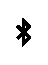
\includegraphics{bluetooth}};
		
		\node[right=40pt of bt1,minimum height=20pt, minimum width=10pt,text width=10pt] (bt2) {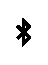
\includegraphics{bluetooth}};
		
		\node[right=10pt of bt2] 			(huvudmodul) 	{Huvudmodul};
		\node[below=-10pt of huvudmodul,draw=none] (master) {\textit{master}};
		\node[right=10pt of huvudmodul] 		(sensormodul) 	{Sensormodul};
		\node[below=-10pt of sensormodul,draw=none] (slave1) {\textit{slav}};
		\node[right=10pt of sensormodul] 	(styrmodul) 		{Styrmodul};
		\node[below=-10pt of styrmodul,draw=none] (slave2) {\textit{slav}};
		
		\coordinate (sclStart) 	at ($(huvudmodul.north west) + (0,20pt)$);
		\coordinate (sclEnd)		at ($(styrmodul.north east)  + (0,20pt)$);
		
		\coordinate (sdaStart)  at ($(sclStart) + (0,20pt)$);
		\coordinate (sdaEnd)		at ($(sclEnd)	+ (0,20pt)$);
		
		\coordinate (vddStart)  at ($(sdaStart) + (0,40pt)$);
		\coordinate (vddEnd)		at ($(sdaEnd)	+ (0,40pt)$);
		
		\draw[thick] (sclStart) -- (sclEnd) node [right,draw=none,text width=0,minimum width=0] {SCL};
		\draw[thick] (sdaStart) -- (sdaEnd) node [right,draw=none,text width=0,minimum width=0] {SDA};
		\draw[thick] (vddStart) -- (vddEnd) node [right,draw=none,text width=0,minimum width=0] {$V_{dd}$};
		
		\draw[thick] (datormodul.east) -- (bt1.west);
		
		\draw[thick, ->,line join=round,decorate, decoration={
    												snake,
    												segment length=5,
    												amplitude=1,
    												post=lineto,
    												post length=1pt}] 
    		($(bt1.east) + (5pt,5pt)$) -- ($(bt2.west) + (-5pt,5pt)$);
    		
    	\draw[thick, ->,line join=round,decorate, decoration={
    												snake,
    												segment length=5,
    												amplitude=1,
    												post=lineto,
    												post length=1pt}] 
    		 ($(bt2.west) + (-5pt,-5pt)$) -- ($(bt1.east) + (5pt,-5pt)$);
    		 
    	\draw[thick] (bt2.east) -- (huvudmodul.west);
    	
    	\draw[thick,fill=black] ($(huvudmodul.north) + (-10pt,0)$) -- ($(huvudmodul.north) + (-10pt,20pt)$) circle [radius=2pt];
    	\draw[thick,fill=black] ($(huvudmodul.north) + (+10pt,0)$) -- ($(huvudmodul.north) + (+10pt,40pt)$) circle [radius=2pt];
    	
    	\draw[thick,fill=black] ($(sensormodul.north) + (-10pt,0)$) -- ($(sensormodul.north) + (-10pt,20pt)$) circle [radius=2pt];
    	\draw[thick,fill=black] ($(sensormodul.north) + (+10pt,0)$) -- ($(sensormodul.north) + (+10pt,40pt)$) circle [radius=2pt];
    	
    	\draw[thick,fill=black] ($(styrmodul.north) + (-10pt,0)$) -- ($(styrmodul.north) + (-10pt,20pt)$) circle [radius=2pt];
    	\draw[thick,fill=black] ($(styrmodul.north) + (+10pt,0)$) -- ($(styrmodul.north) + (+10pt,40pt)$) circle [radius=2pt];
    	
    	\draw[thick,fill=black] ($(sensormodul.north east) + (-5pt,20pt)$) circle [radius=2pt] -- ($(sensormodul.north east) + (-5pt,80pt)$) circle [radius=2pt];
    	\draw[thick,fill=black] ($(styrmodul.north west) + (5pt,40pt)$) circle [radius=2pt] -- ($(styrmodul.north west) + (5pt,80pt)$) circle [radius=2pt];
    	\draw[thick,draw=black,fill=white] ($(styrmodul.north west) + (2pt,50pt)$) rectangle ($(styrmodul.north west) + (8pt,70pt)$);
		\draw[thick,draw=black,fill=white] ($(sensormodul.north east) + (-8pt,50pt)$) rectangle ($(sensormodul.north east) + (-2pt,70pt)$) node [below left=-10pt and 20pt,draw=none,minimum width=0, text width = 0pt] {$R_p$};
		
		\draw[thick, ->] ($(sensormodul.south) + (+40pt,0)$) -- ($(sensormodul.south) + (40pt,-30pt)$) -- ($(huvudmodul.south) + (40pt,-30pt)$) -- ($(huvudmodul.south) + (40pt,0)$);
		\draw[thick, ->] ($(styrmodul.south) + (+40pt,0)$) -- ($(styrmodul.south) + (40pt,-40pt)$) -- node [midway,below,minimum height=20pt, draw=none] {Avbrott}($(huvudmodul.south) + (30pt,-40pt)$) -- ($(huvudmodul.south) + (30pt,0)$);
	\end{tikzpicture}
\end{document}}
	\caption{Intermodulär kommunikation \label{communication}}
\end{figure}

Komponenterna som ingår i robotens huvudmodul är 
\begin{itemize}
  \item[-] Mikroprocessor \verb+ATmega1284p+
  \item[-] Kristalloscillator \verb+EXO-3+ på $14.745$ MHz
  \item[-] Bluetooth\textsuperscript{\circledR}-modul
  \item[-] Resistorer
  \item[-] Kondensator
  \item[-] Studsfri tryckknapp
\end{itemize}

Huvudmodulen är virad på ett virkort enligt kretsschemat i appendix J och är monterat på robotens chassi. 

Nedan beskrivs huvudmodulens olika uppgifter.

\subsubsection{Mjukvara}
I huvudmodulen ingår följande mjukvara:

\begin{description}[style=unboxed, leftmargin=0cm]
  \item[huvudMain.c] som innehåller \textit{main}-funktionen, I\textsuperscript{2}C-kommunikationen och Bluetooth\textsuperscript{\circledR}-kommunikationen. I huvudloopen är det endast styrläget som uppdateras.
%  \item[bluetooth.h] som är ett paket för Bluetooth\textsuperscript{\circledR}-kommunikationen.
  \item[I2C\_master.h] som är ett paket för masterenheten på I\textsuperscript{2}C-bussen.
  \item[searchPath.h] som är ett paket som hanterar avsökning, kartläggning och beräkning av kortaste väg.
\end{description}

\subsubsection{Styrläge}
Det finns två olika styrlägen för roboten, ett autonomt och ett manuellt läge. Rent hårdvarumässigt styrs detta med hjälp av en brytare kopplad till huvudmodulen. När det autonoma läget är aktiverat tas körbeslut utifrån en avsökningsalgoritm som i grunden använder sig av väggföljning av högertyp och \emph{dead-end filling}. Beslutet om vilken kartmodul som ska besökas härnäst baseras på datan som skickas från sensormodulen och på den interna kartläggningen. Detta förklaras närmare i avsnitt \ref{search} och \ref{shortestPath}. När beslutet är taget skickas motsvarande kommando till styrmodulen som sedan utför önskad operation. Ett nytt beslut tas när styrmodulen anser sig vara färdig med nuvarande kommando och begär ett nytt genom avbrott. Hela kommunikationsflödet i autonomt läge finns beskrivet i figur \ref{autonomousMode}. I manuellt läge skickas styrkommandon från datormodulen, via Bluetooth\textsuperscript{\circledR}, till huvudmodulen som sedan vidarebefordrar dessa till styrmodulen. Informationen som skickas baseras på vilken piltangent på datormodulen som är nedtryckt enligt flödet i figur \ref{manualMode}.

\begin{figure}[htbp]
\centering
\noindent\resizebox{0.9\linewidth}{!}{
	\documentclass[border=10px]{standalone}
\usepackage{tikz}
\usetikzlibrary{patterns}
\usetikzlibrary{shapes.geometric}
\usetikzlibrary{shapes.arrows}
\usepackage{amssymb}
\usetikzlibrary{calc}
\usepackage{verbatim}

\pagestyle{empty}
\begin{document}

\tikzstyle{decision} = [diamond, draw,
    text width=5em, text badly centered, node distance=3cm, inner sep=0pt]
    
\tikzstyle{block} = [rectangle, draw,
    text width=7em, text centered, rounded corners, minimum height=4em]
	
\begin{tikzpicture}[scale=1]

%http://www.texample.net/tikz/examples/simple-flow-chart/

\node[block](start){Start};
\node[block, below of = start, node distance = 3cm](nyModul){Välj ny modul att utforska};
\node[block, right of = nyModul, node distance = 5cm](styrning){Skicka styrkommando till styrmodulen};
%\node[block, right of = styrning, node distance = 4.5cm](sensor){Meddela sensormodulen vilken sensordata som önskas till regleringen};
\node[decision, aspect=1.5,right of = styrning, node distance = 4.5cm](regleringKlar){Är regleringen klar?};
\node[block, right of=regleringKlar, node distance = 4.5cm] (sensorData) {Skicka sensordata till styrmodul};

\draw[->](start) -- (nyModul);
\draw[->](nyModul.east) -- (styrning);
\draw[->](styrning) -- (regleringKlar);
%\draw[->](sensor) -- (regleringKlar);
\draw[->](regleringKlar.east) -- node[above]{nej} (sensorData);
\draw[->](sensorData.north) -| ++(0,1.5) node(lowerright){} -| (regleringKlar.north);
\draw[->](regleringKlar.south) -| ++(0,-1.5) node[above right]{ja} -| (nyModul.south);

	\end{tikzpicture}
	
\end{document}
}
	\cprotect\caption{Flödesschema som beskriver förloppet vid autonom styrning \label{autonomousMode}}	
\end{figure}

\begin{figure}[htbp]
\centering
\noindent\resizebox{0.9\linewidth}{!}{
	\documentclass[border=10px]{standalone}
\usepackage{tikz}
\usetikzlibrary{patterns}
\usetikzlibrary{shapes.geometric}
\usetikzlibrary{shapes.arrows}
\usepackage{amssymb}
\usetikzlibrary{calc}
\usepackage{verbatim}

\pagestyle{empty}
\begin{document}

\tikzstyle{decision} = [diamond, draw,
    text width=4em, text badly centered, node distance=3cm, inner sep=0pt]
    
\tikzstyle{block} = [rectangle, draw,
    text width=5em, text centered, rounded corners, minimum height=4em]
	
\begin{tikzpicture}[scale=1]

%http://www.texample.net/tikz/examples/simple-flow-chart/

\node[block](start){Start};
%\node[decision, aspect=2, text width = 8em, below of = start, node distance = 3cm](kommando){Matar användare in styrkommando på tangentbordet?};
\node[block, below of = start, node distance = 3cm, text width = 7em](blåtand){Styrkommando från datormodulen tas emot};
\node[block, right of = blåtand, node distance = 3.5cm, text width = 7em](toStart){Styrkommando skickas från huvudmodul till styrmodul};
\node[decision, aspect=2, text width = 5em, right of = toStart, node distance = 4.5cm](isDone){Har knappen släppts upp?};
\node[block, below of = isDone,node distance = 8em](stop){Skicka stoppsignal till styrmodulen};

\draw[->](start) --  (blåtand);
\draw[->](blåtand) -- (toStart);
\draw[->](toStart) -- (isDone);
\draw[->](isDone) -- node[near start, right]{ja}(stop);
\draw[->](isDone.east) -| node[near start, below]{nej} ++(0.7,2) -| (isDone.north);

	\end{tikzpicture}
	
\end{document}}
	\cprotect\caption{Flödesschema som beskriver förloppet vid manuell styrning \label{manualMode}}	
\end{figure}

\subsubsection{Intern kartläggning} \label{search}
Den interna kartläggningen sker kontinuerligt allt eftersom roboten utforskar labyrinten. Den interna kartan representeras av ett 31x18 fält där robotens startkoordinater är (16,1) och startriktningen är norrut. I fältet lagras varje ny kartmodul som roboten besöker och var sensorerna har registrerat väggar. Längs den tillryggalagda sträckan får varje kartmodul ett värde som motsvarar den kortaste distansen roboten behöver gå för att ta sig dit (med befintlig avsökningsalgoritm), se figur \ref{map}. Efter varje besökt modul med outforskade vägar skickas de uppdaterade värdena i fältet till datormodulen för uppritning, förutsatt att den är ansluten. Är så ej fallet skickas informationen till datormodulen när anslutning har upprättats. 

Återvändsgränder där mål ej hittas sparas i ett annat 31x18 fält, markerade röda i figur \ref{path}, för att förenkla beräkningen av kortaste väg. 

\begin{figure}[htbp]
\centering
\noindent\resizebox{0.7\linewidth}{!}{
	\documentclass[border=10px]{standalone}
\usepackage{tikz}
\usetikzlibrary{patterns}
\usetikzlibrary{shapes.geometric}
\usetikzlibrary{shapes.arrows}
\usepackage{amssymb}
\usetikzlibrary{calc}
\usepackage{verbatim}
\usetikzlibrary{patterns}
\pagestyle{empty}
\begin{document}
    
\tikzstyle{block} = [rectangle, draw,
    text width=4em, text centered, minimum height=4em]
	
\begin{tikzpicture}[scale=1]

%http://www.texample.net/tikz/examples/simple-flow-chart/

\node[block, pattern=north west lines, pattern color= black](1){};
\node[block, pattern = north west lines, pattern color = black, node distance = 4em, below of = 1](2){};
\node[block, pattern = north west lines, pattern color = black, node distance = 4em, below of = 2](3){};
\node[block, node distance = 4em, below of = 3](4){};
\node[block, pattern = north west lines, pattern color = black, node distance = 4em, below of = 4](5){};
\node[block, node distance = 4em, below of = 5](6){};
\node[block, pattern = north west lines, pattern color = black, node distance = 4em, below of = 6](7){};
\node[block, pattern = north west lines, pattern color = black, node distance = 4em, below of = 7](8){};
\node[block, pattern = north west lines, pattern color = black, node distance = 4em, below of = 8](9){};

\node[block, pattern = north west lines, pattern color = black, node distance = 4.7em, left of = 1](111){};
\node[block, pattern = north west lines, pattern color = black, node distance = 4em, below of = 111](112){};
\node[block, pattern = north west lines, pattern color = black, node distance = 4em, below of = 112](113){};
\node[block, pattern = north west lines, pattern color = black, node distance = 4em, below of = 113](114){};
\node[block, pattern = north west lines, pattern color = black, node distance = 4em, below of = 114](115){};
\node[block, pattern = north west lines, pattern color = black, node distance = 4em, below of = 115](116){};
\node[block, pattern = north west lines, pattern color = black, node distance = 4em, below of = 116](117){};
\node[block, pattern = north west lines, pattern color = black, node distance = 4em, below of = 117](118){};
\node[block, pattern = north west lines, pattern color = black, node distance = 4em, below of = 118](119){};


\node[block, pattern = north west lines, pattern color = black, node distance = 4.7em, right of = 1](11){};
\node[block, node distance = 4em, below of = 11](12){};
\node[block, node distance = 4em, below of = 12](13){};
\node[block, node distance = 4em, below of = 13](14){};
\node[block, pattern = north west lines, pattern color = black, node distance = 4em, below of = 14](15){};
\node[block, node distance = 4em, below of = 15](16){};
\node[block, pattern = north west lines, pattern color = black, node distance = 4em, below of = 16](17){};
\node[block, pattern = north west lines, pattern color = black, node distance = 4em, below of = 17](18){};
\node[block, pattern = north west lines, pattern color = black, node distance = 4em, below of = 18](19){};

\node[block, pattern = north west lines, pattern color = black, node distance = 4.7em, right of = 11](21){};
\node[block, node distance = 4em, below of = 21](22){};
\node[block, pattern = north west lines, pattern color = black, node distance = 4em, below of = 22](23){};
\node[block, node distance = 4em, below of = 23](24){};
\node[block, node distance = 4em, below of = 24](25){};
\node[block, node distance = 4em, below of = 25](26){};
\node[block, node distance = 4em, below of = 26](27){};
\node[block, node distance = 4em, below of = 27](28){};
\node[block, pattern = north west lines, pattern color = black, node distance = 4em, below of = 28](29){};

\node[block, pattern = north west lines, pattern color = black, node distance = 4.7em, right of = 21](31){};
\node[block, node distance = 4em, below of = 31](32){};
\node[block, fill = gray, node distance = 4em, below of = 32](33){};
\node[block, fill = gray, node distance = 4em, below of = 33](34){};
\node[block, pattern = north west lines, pattern color = black, node distance = 4em, below of = 34](35){};
\node[block, pattern = north west lines, pattern color = black, node distance = 4em, below of = 35](36){};
\node[block, pattern = north west lines, pattern color = black, node distance = 4em, below of = 36](37){};
\node[block, node distance = 4em, below of = 37](38){};
\node[block, pattern = north west lines, pattern color = black, node distance = 4em, below of = 38](39){};

\node[block,fill = green, node distance = 4.7em, right of = 31](41){\huge 12};
\node[block, node distance = 4em, below of = 41](42){\huge 11};
\node[block, node distance = 4em, below of = 42](43){\huge 10};
\node[block, node distance = 4em, below of = 43](44){\huge 9};
\node[block, fill = gray, node distance = 4em, below of = 44](45){};
\node[block, node distance = 4em, below of = 45](46){};
\node[block, node distance = 4em, below of = 46](47){};
\node[block, node distance = 4em, below of = 47](48){};
\node[block, pattern = north west lines, pattern color = black, node distance = 4em, below of = 48](49){};

\node[block, pattern = north west lines, pattern color = black, node distance = 4.7em, right of = 41](51){};
\node[block, fill = gray, node distance = 4em, below of = 51](52){};
\node[block, fill = gray, node distance = 4em, below of = 52](53){};
\node[block, node distance = 4em, below of = 53](54){\huge 8};
\node[block, fill = gray, node distance = 4em, below of = 54](55){};
\node[block, node distance = 4em, below of = 55](56){};
\node[block, fill = gray, node distance = 4em, below of = 56](57){};
\node[block, pattern = north west lines, pattern color = black, node distance = 4em, below of = 57](58){};
\node[block, pattern = north west lines, pattern color = black, node distance = 4em, below of = 58](59){};

\node[block, pattern = north west lines, pattern color = black, node distance = 4.7em, right of = 51](61){};
\node[block, fill = gray, node distance = 4em, below of = 61](62){};
\node[block, node distance = 4em, below of = 62](63){\huge 8};
\node[block, node distance = 4em, below of = 63](64){\huge 7};
\node[block, node distance = 4em, below of = 64](65){\huge 8};
\node[block, node distance = 4em, below of = 65](66){\huge 9};
\node[block, node distance = 4em, below of = 66](67){\huge 10};
\node[block, fill = gray, node distance = 4em, below of = 67](68){};
\node[block, pattern = north west lines, pattern color = black, node distance = 4em, below of = 68](69){};

\node[block, pattern = north west lines, pattern color = black, node distance = 4.7em, right of = 61](71){};
\node[block, pattern = north west lines, pattern color = black, node distance = 4em, below of = 71](72){};
\node[block, fill = gray, node distance = 4em, below of = 72](73){};
\node[block, node distance = 4em, below of = 73](74){\huge 6};
\node[block, fill = gray, node distance = 4em, below of = 74](75){};
\node[block, fill = gray, node distance = 4em, below of = 75](76){};
\node[block, node distance = 4em, below of = 76](77){\huge 1};
\node[block, fill = cyan, node distance = 4em, below of = 77](78){\huge 0};
\node[block, pattern = north west lines, pattern color = black, node distance = 4em, below of = 78](79){};

\node[block, pattern = north west lines, pattern color = black, node distance = 4.7em, right of = 71](81){};
\node[block, fill = gray, node distance = 4em, below of = 81](82){};
\node[block, node distance = 4em, below of = 82](83){\huge 6};
\node[block, node distance = 4em, below of = 83](84){\huge 5};
\node[block, node distance = 4em, below of = 84](85){\huge 4};
\node[block, node distance = 4em, below of = 85](86){\huge 3};
\node[block, node distance = 4em, below of = 86](87){\huge 2};
\node[block, fill = gray, node distance = 4em, below of = 87](88){};
\node[block, pattern = north west lines, pattern color = black, node distance = 4em, below of = 88](89){};


\node[block, pattern = north west lines, pattern color = black, node distance = 4.7em, right of = 81](91){};
\node[block, fill = gray, node distance = 4em, below of = 91](92){};
\node[block, node distance = 4em, below of = 92](93){\huge 7};
\node[block, fill = gray, node distance = 4em, below of = 93](94){};
\node[block, fill = gray, node distance = 4em, below of = 94](95){};
\node[block, fill = gray, node distance = 4em, below of = 95](96){};
\node[block, fill = gray, node distance = 4em, below of = 96](97){};
\node[block, fill = gray, node distance = 4em, below of = 97](98){};
\node[block, pattern = north west lines, pattern color = black, node distance = 4em, below of = 98](99){};

\node[block, pattern = north west lines, pattern color = black, node distance = 4.7em, right of = 91](101){};
\node[block, pattern = north west lines, pattern color = black, node distance = 4em, below of = 101](102){};
\node[block, fill = gray, node distance = 4em, below of = 102](103){};
\node[block, pattern = north west lines, pattern color = black, node distance = 4em, below of = 103](104){};
\node[block, pattern = north west lines, pattern color = black, node distance = 4em, below of = 104](105){};
\node[block, pattern = north west lines, pattern color = black, node distance = 4em, below of = 105](106){};
\node[block, pattern = north west lines, pattern color = black, node distance = 4em, below of = 106](107){};
\node[block, pattern = north west lines, pattern color = black, node distance = 4em, below of = 107](108){};
\node[block, pattern = north west lines, pattern color = black, node distance = 4em, below of = 108](109){};


%Top row
\node[block, pattern = north west lines, pattern color = black, node distance = 4em, above of = 1](700){};
\node[block, pattern = north west lines, pattern color = black, node distance = 4.7em, left of = 700](701){};
\node[block, pattern = north west lines, pattern color = black, node distance = 4.7em, right of = 700](702){};
\node[block, pattern = north west lines, pattern color = black, node distance = 4.7em, right of = 702](703){};
\node[block, pattern = north west lines, pattern color = black, node distance = 4.7em, right of = 703](704){};
\node[block, pattern = north west lines, pattern color = black, node distance = 4.7em, right of = 704](705){};
\node[block, pattern = north west lines, pattern color = black, node distance = 4.7em, right of = 705](706){};
\node[block, pattern = north west lines, pattern color = black, node distance = 4.7em, right of = 706](707){};
\node[block, pattern = north west lines, pattern color = black, node distance = 4.7em, right of = 707](708){};
\node[block, pattern = north west lines, pattern color = black, node distance = 4.7em, right of = 708](709){};
\node[block, pattern = north west lines, pattern color = black, node distance = 4.7em, right of = 709](710){};
\node[block, pattern = north west lines, pattern color = black, node distance = 4.7em, right of = 710](711){};
\node[block, pattern = north west lines, pattern color = black, node distance = 4.7em, right of = 711](712){};

\node[block, pattern = north west lines, pattern color = black, node distance = 4.7em, right of = 101](121){};
\node[block, pattern = north west lines, pattern color = black, node distance = 4em, below of = 121](122){};
\node[block, pattern = north west lines, pattern color = black, node distance = 4em, below of = 122](123){};
\node[block, pattern = north west lines, pattern color = black, node distance = 4em, below of = 123](124){};
\node[block, pattern = north west lines, pattern color = black, node distance = 4em, below of = 124](125){};
\node[block, pattern = north west lines, pattern color = black, node distance = 4em, below of = 125](126){};
\node[block, pattern = north west lines, pattern color = black, node distance = 4em, below of = 126](127){};
\node[block, pattern = north west lines, pattern color = black, node distance = 4em, below of = 127](128){};
\node[block, pattern = north west lines, pattern color = black, node distance = 4em, below of = 128](129){};
	\end{tikzpicture}
	
\end{document}
}
	\caption{Schematisk bild av den interna kartan}	\label{map}
\end{figure}

\subsubsection{Beräkning av kortaste väg} \label{shortestPath}
Beräkningen av kortaste vägen till målet sker med utgångspunkt från A\textsuperscript{*}-algoritmen. När målet är funnet numreras varje nod som roboten besöker från målet med en siffra som representerar ett avstånd till målet, se figur \ref{path}. För att inte utforska mer än nödvändigt används en pessimistisk skattning av avståndet från start till mål som jämförelsevärde. Detta värde motsvarar det antal steg robotens första väg från start till mål blev, återvändsgränder borträknat. Under den fortsatta utforskningen av labyrinten jämförs denna skattning med summan av köravståndet från målet, det vill säga värdet den kartmodulen skulle ha i figur \ref{path}, och manhattanavståndet från start till aktuell nod. Är det avståndet lika med eller större än skattningen är det inte nödvändigt att utforska mer åt det hållet och motsvarande modul markeras för att i beräkningen inte ta hänsyn till den riktningen, se orangemarkerade moduler i figur \ref{path}. Skulle en bättre pessimistisk skattning dyka upp på vägen uppdateras värdet för att ytterligare minska ned antalet moduler som måste besökas.

\begin{figure}[htbp]
\centering
\noindent\resizebox{0.7\linewidth}{!}{
	\documentclass[border=10px]{standalone}
\usepackage{tikz}
\usetikzlibrary{patterns}
\usetikzlibrary{shapes.geometric}
\usetikzlibrary{shapes.arrows}
\usepackage{amssymb}
\usetikzlibrary{calc}
\usepackage{verbatim}

\pagestyle{empty}
\begin{document}
    
\tikzstyle{block} = [rectangle, draw,
    text width=4em, text centered, minimum height=4em]
	
\begin{tikzpicture}[scale=1]

%http://www.texample.net/tikz/examples/simple-flow-chart/

\node[block, fill = black](1){};
\node[block, fill = black, node distance = 4em, below of = 1](2){};
\node[block, fill = black, node distance = 4em, below of = 2](3){};
\node[block, node distance = 4em, below of = 3](4){};
\node[block, fill = black, node distance = 4em, below of = 4](5){};
\node[block, node distance = 4em, below of = 5](6){};
\node[block, fill = black, node distance = 4em, below of = 6](7){};
\node[block, fill = black, node distance = 4em, below of = 7](8){};
\node[block, fill = black, node distance = 4em, below of = 8](9){};

\node[block, fill = black, node distance = 4.7em, left of = 1](111){};
\node[block, fill = black, node distance = 4em, below of = 111](112){};
\node[block, fill = black, node distance = 4em, below of = 112](113){};
\node[block, fill = black, node distance = 4em, below of = 113](114){};
\node[block, fill = black, node distance = 4em, below of = 114](115){};
\node[block, fill = black, node distance = 4em, below of = 115](116){};
\node[block, fill = black, node distance = 4em, below of = 116](117){};
\node[block, fill = black, node distance = 4em, below of = 117](118){};
\node[block, fill = black, node distance = 4em, below of = 118](119){};


\node[block, fill = black, node distance = 4.7em, right of = 1](11){};
\node[block, node distance = 4em, below of = 11](12){};
\node[block, node distance = 4em, below of = 12](13){};
\node[block, node distance = 4em, below of = 13](14){};
\node[block, fill = black, node distance = 4em, below of = 14](15){};
\node[block, node distance = 4em, below of = 15](16){};
\node[block, fill = black, node distance = 4em, below of = 16](17){};
\node[block, fill = black, node distance = 4em, below of = 17](18){};
\node[block, fill = black, node distance = 4em, below of = 18](19){};

\node[block, fill = black, node distance = 4.7em, right of = 11](21){};
\node[block, node distance = 4em, below of = 21](22){};
\node[block, fill = black, node distance = 4em, below of = 22](23){};
\node[block, node distance = 4em, below of = 23](24){};
\node[block, node distance = 4em, below of = 24](25){};
\node[block, node distance = 4em, below of = 25](26){};
\node[block, node distance = 4em, below of = 26](27){};
\node[block, node distance = 4em, below of = 27](28){};
\node[block, fill = black, node distance = 4em, below of = 28](29){};

\node[block, fill = black, node distance = 4.7em, right of = 21](31){};
\node[block, fill = red, node distance = 4em, below of = 31](32){};
\node[block, fill = black, node distance = 4em, below of = 32](33){};
\node[block, fill = black, node distance = 4em, below of = 33](34){};
\node[block, fill = black, node distance = 4em, below of = 34](35){};
\node[block, fill = black, node distance = 4em, below of = 35](36){};
\node[block, fill = black, node distance = 4em, below of = 36](37){};
\node[block, node distance = 4em, below of = 37](38){};
\node[block, fill = black, node distance = 4em, below of = 38](39){};

\node[block,fill = green, node distance = 4.7em, right of = 31](41){\huge 0};
\node[block, node distance = 4em, below of = 41](42){\huge 1};
\node[block, node distance = 4em, below of = 42](43){\huge 2};
\node[block, node distance = 4em, below of = 43](44){\huge 3};
\node[block, fill = black, node distance = 4em, below of = 44](45){};
\node[block, node distance = 4em, below of = 45](46){};
\node[block, node distance = 4em, below of = 46](47){};
\node[block, node distance = 4em, below of = 47](48){};
\node[block, fill = black, node distance = 4em, below of = 48](49){};

\node[block, fill = black, node distance = 4.7em, right of = 41](51){};
\node[block, fill = black, node distance = 4em, below of = 51](52){};
\node[block, fill = black, node distance = 4em, below of = 52](53){};
\node[block, node distance = 4em, below of = 53](54){\huge 4};
\node[block, fill = black, node distance = 4em, below of = 54](55){};
\node[block, fill = red, node distance = 4em, below of = 55](56){};
\node[block, fill = black, node distance = 4em, below of = 56](57){};
\node[block, fill = black, node distance = 4em, below of = 57](58){};
\node[block, fill = black, node distance = 4em, below of = 58](59){};

\node[block, fill = black, node distance = 4.7em, right of = 51](61){};
\node[block, fill = black, node distance = 4em, below of = 61](62){};
\node[block, fill = red, node distance = 4em, below of = 62](63){};
\node[block, node distance = 4em, below of = 63](64){\huge 5};
\node[block, node distance = 4em, below of = 64](65){\huge 6};
\node[block, node distance = 4em, below of = 65](66){\huge 7};
\node[block, node distance = 4em, below of = 66](67){\huge 8};
\node[block, fill = black, node distance = 4em, below of = 67](68){};
\node[block, fill = black, node distance = 4em, below of = 68](69){};

\node[block, fill = black, node distance = 4.7em, right of = 61](71){};
\node[block, fill = black, node distance = 4em, below of = 71](72){};
\node[block, fill = black, node distance = 4em, below of = 72](73){};
\node[block, node distance = 4em, below of = 73](74){\huge 6};
\node[block, fill = black, node distance = 4em, below of = 74](75){};
\node[block, fill = black, node distance = 4em, below of = 75](76){};
\node[block, node distance = 4em, below of = 76](77){\huge 11};
\node[block, fill = cyan, node distance = 4em, below of = 77](78){\huge 12};
\node[block, fill = black, node distance = 4em, below of = 78](79){};

\node[block, fill = black, node distance = 4.7em, right of = 71](81){};
\node[block, fill = black, node distance = 4em, below of = 81](82){};
\node[block, fill = red, node distance = 4em, below of = 82](83){};
\node[block, node distance = 4em, below of = 83](84){\huge 7};
\node[block, node distance = 4em, below of = 84](85){\huge 8};
\node[block, node distance = 4em, below of = 85](86){\huge 9};
\node[block, node distance = 4em, below of = 86](87){\huge 10};
\node[block, fill = black, node distance = 4em, below of = 87](88){};
\node[block, fill = black, node distance = 4em, below of = 88](89){};


\node[block, fill = black, node distance = 4.7em, right of = 81](91){};
\node[block, fill = black, node distance = 4em, below of = 91](92){};
\node[block, node distance = 4em, below of = 92](93){};
\node[block, fill = black, node distance = 4em, below of = 93](94){};
\node[block, fill = black, node distance = 4em, below of = 94](95){};
\node[block, fill = black, node distance = 4em, below of = 95](96){};
\node[block, fill = black, node distance = 4em, below of = 96](97){};
\node[block, fill = black, node distance = 4em, below of = 97](98){};
\node[block, fill = black, node distance = 4em, below of = 98](99){};

\node[block, fill = black, node distance = 4.7em, right of = 91](101){};
\node[block, fill = black, node distance = 4em, below of = 101](102){};
\node[block, fill = black, node distance = 4em, below of = 102](103){};
\node[block, fill = black, node distance = 4em, below of = 103](104){};
\node[block, fill = black, node distance = 4em, below of = 104](105){};
\node[block, fill = black, node distance = 4em, below of = 105](106){};
\node[block, fill = black, node distance = 4em, below of = 106](107){};
\node[block, fill = black, node distance = 4em, below of = 107](108){};
\node[block, fill = black, node distance = 4em, below of = 108](109){};


%Top row
\node[block, fill = black, node distance = 4em, above of = 1](700){};
\node[block, fill = black, node distance = 4.7em, left of = 700](701){};
\node[block, fill = black, node distance = 4.7em, right of = 700](702){};
\node[block, fill = black, node distance = 4.7em, right of = 702](703){};
\node[block, fill = black, node distance = 4.7em, right of = 703](704){};
\node[block, fill = black, node distance = 4.7em, right of = 704](705){};
\node[block, fill = black, node distance = 4.7em, right of = 705](706){};
\node[block, fill = black, node distance = 4.7em, right of = 706](707){};
\node[block, fill = black, node distance = 4.7em, right of = 707](708){};
\node[block, fill = black, node distance = 4.7em, right of = 708](709){};
\node[block, fill = black, node distance = 4.7em, right of = 709](710){};
\node[block, fill = black, node distance = 4.7em, right of = 710](711){};
	\end{tikzpicture}
	
\end{document}}
	\caption{Schematisk bild av kartan för beräkning av kortaste väg}	\label{path}
\end{figure}


Kortaste väg från start till mål fås då genom att, för varje nod, välja den närliggande nod med lägst siffra enligt figur \ref{path}. De orange- och rödmarkerade kartmodulerna är implementerade med högre siffror än vad roboten skulle kunna köra  enligt tävlingsreglerna, se appendix B.

\pagebreak

\subsection{Sensormodulen}
Robotens sensormodul har som uppgift att läsa av sensorerna och kommunicera datan till huvudmodulen. De sensorer som används och placeringar av dessa illustreras i figur \ref{sensors}.
\newline
%\begin{description}
%	\item[Avstånd] \hfill \\
%	4 x IR-sensor \verb+GP2D120+ (4 cm till 30 cm) \\
%	1 x Laser-sensor \verb+LIDAR-Lite v2+ (0 till 40 m) \\
%	\item[Vinkelhastighet] \hfill \\
%	1 x Gyro/accelerometer \verb+MLX90609+ 
%	\item[Identifierare av nödställd] \hfill \\
%	1 x IR-detektor \verb+IRM-8601-S+
%\end{description}
%Figur \ref{sensors} illustrerar placeringen av, de ovan angivna, sensorerna. 

\begin{figure}[htbp]
\centering
\noindent\resizebox{.8\textwidth}{!}{
	\documentclass[border=10px]{standalone}
\usepackage{tikz}
\usetikzlibrary{patterns}
\usetikzlibrary{shapes.arrows}
\usepackage{amssymb}
\usetikzlibrary{calc}
\usepackage{verbatim}
\begin{document}
	
\begin{tikzpicture}[scale=1,rotate=90]
		
	%Base
	\draw[thick, draw=black, fill=gray!10] (0,0) rectangle (6,10);

	%Wheels
	\draw[thick, pattern=north west lines, pattern color=black] (-.5,1) 		rectangle (0,2.5);
	\draw[thick, pattern=north west lines, pattern color=black] (-.5,7.5) 	rectangle (0,9);
	\draw[thick, pattern=north west lines, pattern color=black] (6,1) 		rectangle (6.5,2.5);
	\draw[thick, pattern=north west lines, pattern color=black] (6,7.5) 		rectangle (6.5,9);
	
	%Sensors
	\draw[thick, draw=black, fill=white] (-.25,.25) 		rectangle (.5,.75);
	\draw[thick, draw=black, fill=white] (-.25,9.25) 	rectangle (.5,9.75);
	\draw[thick, draw=black, fill=white] (5.5,.25) 		rectangle (6.25,.75);
	\draw[thick, draw=black, fill=white] (5.5,9.25) 		rectangle (6.25,9.75);
	\draw[thick, draw=black, fill=white] (2,10.25) 		rectangle (4,9.5);
	\draw[thick, draw=black, fill=white] (2.5,4) 		rectangle (3.5,6);
	
	%Arrows and text
	\draw[thick, ->]  (3,11) node[left, align=center] {\verb+LIDAR-Lite v2+ \\ + detektor av nödställd} -- (3,10.25);
	\draw[thick, <->] (0.5,0.5)  --  (5.5,0.5) node[left=-14pt,midway, fill=gray!10] {\verb+GP2D120+};
	\draw[thick, <->] (0.5,9.5) -- (3,9) node[right=-14pt,fill=gray!10] {\verb+GP2D120+} -- (5.5,9.5);
	\draw[thick, ->] (4.5,5) node[above] {\verb+MLX90609+} -- (3.5,5);
	\end{tikzpicture}
	
\end{document}	}
	\caption{Sensorplacering \label{sensors}}
\end{figure}

De komponenter som utöver sensorerna ingår i robotens sensormodul är följande:
\begin{itemize}
  \item[-] Mikroprocessor \verb+ATmega1284p+
  \item[-] Kristalloscillator \verb+EXO-3+ med $16$ MHz frekvens
  \item[-] Resistorer
  \item[-] Kondensator
  \item[-] Lågpassfilter
  \item[-] Studsfri tryckknapp
\end{itemize}

Sensormodulen är ihopkopplad enligt kopplingsschema i appendix J. Den är sammankopplad på ett separat virkort, som är monterat på robotens chassi. Nedan följer utförligare beskrivningar av sensormodulens hårdvara, mjukvara och gränssnitt.

\subsubsection{Mjukvara}
I sensormodulen ingår följande mjukvara: 

\begin{description}[style=unboxed, leftmargin=0cm]
  \item[sensorModule.c] som innehåller modulens \textit{main}-funktion, i vilken omvandling av sensorvärden till SI-enhet sker. Den innehåller dessutom kod för I\textsuperscript{2}C-kommunikation mellan modulerna. I main-funktionens huvudloop läggs de omvandlade sensorenheterna in i ett fält, vilket senare kommuniceras till huvudmodulen.
  \item[sensorInit.h] som är ett paket som initierar de olika gränssnitten för överföring av sensordata mellan mikroprocessorn och de olika sensorerna.
  \item[I2C\_slave.h] som är ett paket för slavarna inom I\textsuperscript{2}C-bussen, lämpligt i detta fall då sensormodulen är slav i kommunikationen med huvudmodulen.
\end{description}

\subsubsection{\texttt{Lidar-Lite v2}, avståndssensor}
För att mäta avstånd framåt används lasersensorn \verb+Lidar-Lite v2+. Den sänder ut en laserpuls och mäter tiden det tar för denna att reflekterats och återvända. På så sätt kan avstånd upp till $40$ meter uppmätas med en felmarginal på $2,5$ centimeter. Den kan dock ge felaktiga värden när den opererar i en omgivning som labyrinten. Det beror på att det finns en risk att sensorn mäter avstånd till en sidokorridor, när den tror att den mäter avståndet till väggen rakt fram.

Kommunikationen av sensordata mellan \verb+Lidar-Lite v2+ och mikroprocessorn \verb+ATmega1284p+ sker via pulsbreddsmodulering. Längden på pulsbreddens positiva flank är proportionell mot sensorns avstånd till närmaste föremål, vilket gör omvandligen till SI-enhet enkel. För att mäta pulsbredden kopplas lasersensorns trigger pin till en av mikroprocessorns externa avbrottsingångar, se kopplingsschema i Appendix J. 

\subsubsection{\texttt{SFH300}, reflexsensor}
För att komplettera avståndsmätningen används även en reflexsensor av modell \verb+SFH300+. Sensorn sänder ut ljus och mäter hur mycket av ljuset som reflekteras. Genom att fästa en skiva indelad i 16 lika stora tårtbitar, varannan vit och varannan svart, på ett av hjulen kan tillryggalagt avstånd bestämmas.

Hjulens omkrets kan mätas och därefter divideras med 16. På så sätt erhålls hur långt roboten åker per tårtbit.
Då utsignalen är analog krävs AD-omvandling, varefter ett digitalt värde mellan 0 och 255 erhålls. Genom experiment kan ett lämpligt referensvärde hittas där värden över detta tolkas som svart yta och lägre värden tolkas som vit yta. Detta fungerar eftersom vita ytor reflekterar mycket mer ljus än vad svarta ytor gör. Genom att räkna hur många ljusskiftningar som har skett kan sedan tillryggalagt avstånd erhållas.

\subsubsection{\texttt{GP2D120}, avståndssensor}
För att mäta avståndet till sidoväggarna används fyra IR-sensorer av modell \verb+GP2D120+. Avståndet mäts genom att IR-ljus med en viss våglängd skickas ut från sensorn, reflekteras mot väggarna för att sedan detekteras av sensorn. Genom att mäta den vinkel reflektionen sker med kan avståndet till väggen bedömas. Utsignalen är analog i form av spänning och behöver lågpassfiltreras på grund av mängden högfrekvent brus i signalen. Lågpassfiltreringen sker genom att leda signalen genom en RC-krets. 

Portarna A0-A7 på \verb+ATmega1284p+ kan användas som AD-omvandare, vilket utnyttjas för att generera ett digitalt värde. Det digitala värdet är inte linjärt beroende av avståndet utan sambandet beskrivs av en tredjegradsfunktion. Genom empiriska tester kan funktionen bestämmas tillräckligt bra för att ge värden att reglera på.

\subsubsection{\texttt{MLX90609}, gyro}
För att kunna utföra lagom stor rotation vid svängar används gyrot \verb+MLX90609+ som mäter den momentana vinkelhastigheten. Att bestämma hur många grader roboten roterar görs genom att summera värdet på vinkelhastigheten med tillräckligt hög samplingsfrekvens, vilket motsvarar integrering av vinkelhastigheten. Kommunikation av informationen mellan sensorn och mikroprocessorn sker via ett SPI-gränssnitt, där mikroprocessorn fungerar som SPI-master. Vinkelhastigheten representeras av elva bitar men kapas till åtta innan informationen kommuniceras vidare. Då de tre minst signifikanta bitarna tas bort blir precisionen något sämre men informationen rymms på en byte. Tester kan sedan genomföras för att bestämma vilket värde som motsvarar en grads rotation.  

\subsubsection{\texttt{IRM-8601-S}, IR-detektor}
Då den nödställde sänder ut en IR-signal krävs identifikation av ett specifikt bitmönster. För detta ändamål används IR-detektorn \verb+IRM-8601-S+. Bitmönstret identifieras genom att ansluta insignalen till en extern avbrottsingång på mikroprocessorn. TIMER0 används därefter för att räkna tiden på de höga bitarna hos insignalen som IR-detektorn identifierar. Stämmer tiden för de höga bitarna överens med det bitmönster som den nödställde ska sända ut är den nödställde funnen.

\subsection{Styrmodulen}

Styrmodulen är den del av roboten som tar emot och verkställer styrkommandon och ser till att roboten tar sig fram på önskat sätt. Det som hanteras är styrning av chassits motorer för att få roboten att röra på sig och att styra gripklon. 

De komponenter som ingår i styrmodulen är
\begin{itemize}
  \item[-] Mikroprocessor \verb+ATmega1284p+
  \item[-] LCD-display \verb+JM162A+
  \item[-] Kristalloscillator \verb+EXO-3+ på $16$ MHz
  \item[-] LED-dioder
  \item[-] Resistorer
  \item[-] Kondensator
  \item[-] Potentiometer
  \item[-] Studsfri tryckknapp
\end{itemize}

Styrmodulen kopplas enligt kretsschemat i appendix J. Kopplingen sker på ett virkort som sedan monteras på robotens chassi. Härefter följer detaljerade beskrivningar av styrmodulens olika delar.

\subsubsection{Mjukvara}
Mjukvaran till styrmodulen består av följande filer:
\begin{description}[style=unboxed, leftmargin=0cm]
  \item[controlModule.c] som innehåller \textit{main}-funktionen, I\textsuperscript{2}C-kommunikationen och regleringen. I huvudloopen är den endast LCD-displayen och LED-dioderna som uppdateras.
  \item[PWM.h] som är ett paket för pulsbreddsmodulering.
  \item[LCD.h] som är ett paket för LCD-displayen.
  \item[constants.h] som är ett paket med definitioner av konstanter till controlModule.c.
  \item[I2C\_slave.h] som är ett paket för slavar inom I\textsuperscript{2}C-bussen.

\end{description}


\subsubsection{PWM}
Pulsbreddsmodulering används för att styra respektive hjulpar, gripklon och servot för den främre sensorn. På \verb+ATMega1284p+ har varje timer två utgångar, utgång A och B. En timer kopplas således till båda hjulparen så att de delar samma inställningar gällande frekvens och periodtid men styrs med olika arbetscykler. Gripklon och servot för den främre sensorn delar i sin tur även samma egenskaper och tilldelas en gemensam timer. Samtliga timers som används är av 16-bitarstyp, men alla bitar behövs inte och därför utnyttjas möjligheten att konfigurera om dem så att enbart de nödvändiga används. Nedan finns konfigurationerna beskrivna mer detaljerat. 

\begin{center}
\begin{tabular}{l l l l l}

    \textbf{Syfte} & \textbf{Läge} & \textbf{Antal bitar} & \textbf{Prescale} & \textbf{Toppvärde} \\
    Hjulpar & Fast PWM, 10-bit & 10 bitar & $\text{clk}/64$ &  0x03FF \\
	Gripklo och sensorservo & Fast PWM & 16 bitar & $\text{clk}/64$  & ICR \\
\end{tabular}
\end{center}

\subsubsection{LCD-display}
LCD-displayen, \verb+JM162A+, består av två rader där respektive har plats för 16 tecken. På displayen visas sensordata under robotens färd som uppdateras i takt med att nya sensordata anländer. En potentiometer kopplas in för att justera kontrastspänningen och LCD:n konfigureras enligt nedan.

\begin{center}
  \begin{tabular}{l l l l l l l l}
      \textbf{Modell} & \textbf{Bitar} & \textbf{Rader} & \textbf{Punkter} & \textbf{Pekare} & \textbf{Blink} & \textbf{Öka pekare} & \textbf{Skifta text} \\
      \verb+JM162A+ & 8 & 2 & 5x7 & Av & Av & På & Av \\
    \end{tabular}
  \end{center}

\subsubsection{Styrlägen}
Styrmodulen har två olika styrlägen: autonomt eller manuellt läge.
\begin{description}[style=unboxed, leftmargin=0cm]
  \item[Autonomt läge]
    I autonomt läge agerar styrmodulen på beslut som tas från huvudmodulen. Målet är att navigera modulvis genom den avsökningalgoritm som är implementerad på huvudmodulen. Styrmodulen begär ett nytt styrkommando genom att skicka en positiv flank på en utgång som är kopplad till ett avbrott hos huvudmodulen. Huvudmodulen tar därefter ett beslut om vilket styrkommando som ska skickas. De möjliga styrkommandona är \textit{Fram}, \textit{Halv fram}, \textit{Halv bak}, \textit{Rotera 90\textdegree\ vänster}, \textit{Rotera 90\textdegree\ höger}, \textit{Rotera 180\textdegree} och \textit{Stopp}. 

När ett styrkommando tas emot av styrmodulen sker regleringen i samband med inkommande sensordata. För att regleringen ska agera snabbt nog behöver sensordata skickas i takten $30$ Hz. När sensordata tas emot sparas samtliga värden lokalt i styrmodulen. Därefter kallas den metod som sköter reglering av styrkommandot. 

Styrkommandot \textit{Fram} innebär att roboten ska flytta sig en modul föröver. Modullängden är densamma för hela banan och satt till $40$ centimeter. Roboten beräknar tillryggalagd sträcka genom att beräkna antalet varv hjulen roterar och under färden sker reglering enligt avsnitt \ref{subsection:reglering}. När modulen är avverkad kallas återigen huvudmodulen för ett nytt styrkommando. Tack vare hastigheten hos I\textsuperscript{2}C-bussen och fördröjningen hos PWM-styrningen agerar roboten på nästa kommando utan ett ryck emellan. 

Styrkommandot \textit{Halv fram} tas emot när roboten befinner sig framför målet och ska lämna förnödenheten. Styrmodulen agerar på samma sätt som vid kommandot \textit{Fram} fast med halverad önskad sträcka. När styrkommandot tas emot sparas främre sensorns värde, för att sedan jämföras med i nästa styrkommando, se nedan.

Styrkommandot \textit{Halv bak} tas alltid emot efter ett kommando av typen \textit{Halv fram}. Båda hjulparen drivs bakåt och roboten jämför det främre sensorvärdet med det som sparades vid \textit{Halv fram}, för att försäkra sig om att den är tillbaka en halv modul. 

Styrkommandot \textit{Rotera 90\textdegree\ vänster/höger} innebär en vinkelrät rotation åt respektive håll. Här förutsätts roboten befinna sig mitt i en modul och behöver med andra ord inte reglera sig i vertikal- eller horisontellt led. Regleringen av rotation sker med hjälp av det gyro som förmedlar vinkelhastighet till sensormodulen. När en rotation påbörjas summeras vinkelhastigheterna hos styrmodulen i takt med varenda nytt sensordata. Nivån som summationen sker till byter endast tecken mellan vänster- och högerrotation. Det är rotationsregleringen som sätter kravet att sensordata ska skickas med $30$ Hz för att minimera felet vid snabba rotationer. 

Styrkommandot \textit{Rotera 180\textdegree} innebär ett halvt varvs rotation av roboten. Regleringen sker på samma sätt som den vinkelräta rotationen. Den enda skillnaden är det tak summationen sker till. 

För att hantera det sensorfel som gyrot för med sig följer ytterligare en reglering efter båda typerna av rotation. Regleringen bygger på att det finns en vägg att förhålla sig till och kallas därför inte om roboten befinner sig i en fyrvägskorsning. När det finns en vägg på någon sida rätar roboten upp sig genom att minimera differensen mellan den främre och bakre sensorn. 

Stykommandot \textit{Stopp} innebär att båda hjulparen stannas och ingen reglering sker. 

\item[Manuellt läge] I manuellt läge styrs roboten via styrkommandon från datormodulen. När styrmodulen tar emot ett styrkommando och befinner sig i detta läge sker körningen helt utan reglering. 

Styrmodulen fortsätter med samma styrkommando tills nästa har skickats. Med andra ord krävs det ett stoppkommando för att stanna roboten. Stoppkommandot skickas per automatik när datormodulens piltangent har släppts upp och behöver därför inte tas hänsyn till av användaren. 

När ett styrkommando skickas till styrmodulen i manuellt läge tolkas den tredje byten i sändningen som den önskade hastigheten. Hastigheten tas emot som ett heltal i intervallet noll till 100. Det skalas därefter till motsvarande intervall för pulsbreddsmoduleringen.

  \end{description}

\subsection{Datormodulen}
Datormodulen är skriven i Java och följer desingmönstret model-view-controller. Modulen har två huvudsakliga syften. Det ena är att skicka data till roboten, för att kunna styra den manuellt och på ett enkelt sätt ändra olika inställningar hos roboten. Det andra är att ta emot data från roboten för att presentera robotens omgivning i form av sensorvärden och kartdata. Nedan följer en beskrivning av programmets tre delar. Utöver dessa delar finns en del stödklasser, bland annat för hantering av konstanter och text.%Förklara m-v-c?

\subsubsection{Model}
``Model''-delen av programet består av fyra huvudsakliga klasser: Log, RobotData, SensorData och MapData. 
Log-klassen används för att spara ner relevanta händelser under testkörningar till txt-filer. 
RobotData-klassen tar hand om den interna representationen av robotens tillstånd, det vill säga robotens nuvarande körläge, senast skickade körkommando med mera. 
SensorData-klassen sparar de senast mottagna sensorvärdena från roboten. 
MapData-klassen sparar alla mottagna kartdata från roboten. De sistnämnda tre data-klasserna används också för att, genom observatörer, ändra den grafiska ``view''-delen av programmet.

\subsubsection{View}
``View''-delen av programmet sköter programmets grafiska användargränssnitt och består av sex huvudsakliga klasser: Animator, MenuBar, MapPanel, GraphPanel, TablePanel och RobotStatusPanel. Animator-klassen samordnar de olika grafiska elementen och sköter instansieringen av användargränssnittet. 
MenuBar-klassen hanterar menyn i huvudfönstret. Genom den kan användaren välja körläge, hantera loggar och komma åt hjälpmenyn. 
MapPanel-klassen sköter den grafiska representationen av kartan. Varje sektion av kartan representeras med ett visuellt element med olika färg beroende på om det är en vägg, start, mål eller en vanlig ruta. Kartan expanderas dynamiskt allteftersom roboten utforskar sin omgivning. 
GraphPanel-klassen presenterar historiska sensordata i grafer och använder sig av det publika biblioteket JFreeChart 1.0.19. 
TablePanel-klassen presenterar de senast mottagna sensorvärdena i en tabell. Denna klass låter även användaren ändra vissa reglerkonstanter hos roboten i vissa lägen.
RobotStatusPanel-klassen visar robotens nuvarande status, det vill säga autonomt eller manuellt läge, det senast skickade styrkommandot med mera.

\begin{figure}[H]
\centering
\noindent\resizebox{.8\linewidth}{!}{
	\documentclass[border=10px]{standalone}
\usepackage{tikz}
\usetikzlibrary{patterns}
\usetikzlibrary{shapes.arrows}
\usepackage{amssymb}
\usetikzlibrary{calc}
\usepackage{verbatim}
\usepackage[swedish]{babel}
\begin{document}
	
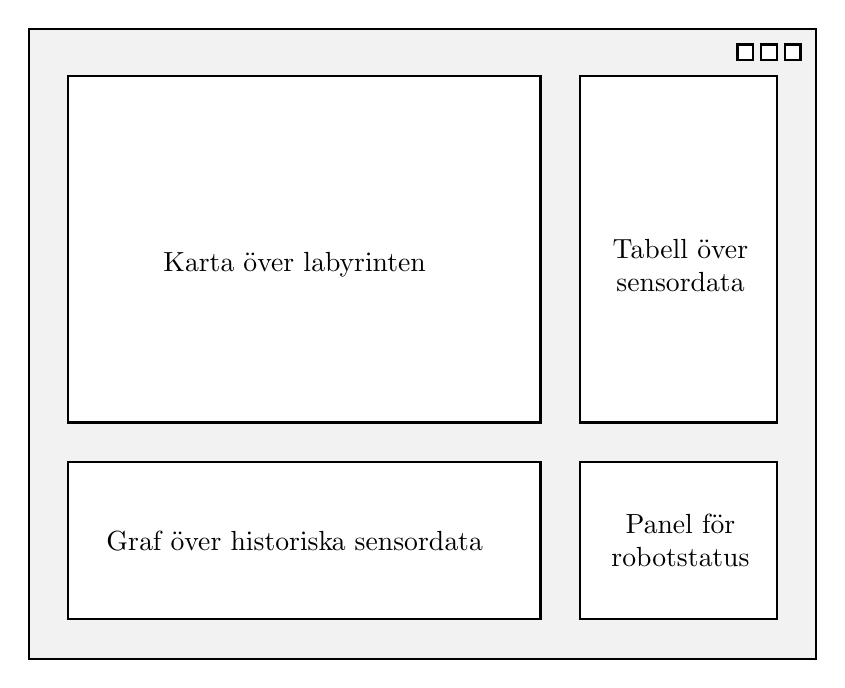
\begin{tikzpicture}[scale=1,rotate=0]
		
	%Frame
	\draw[thick, draw=black, fill=gray!10] (0,0) rectangle (10,8);

	%Exit and minimize
	\draw[thick, draw=black, fill=white] (9.0,7.6) rectangle (9.2,7.8);
	\draw[thick, draw=black, fill=white] (9.3,7.6) rectangle (9.5,7.8);
	\draw[thick, draw=black, fill=white] (9.6,7.6) rectangle (9.8,7.8);
	
	%Map
	\draw[thick, draw=black, fill=white] (0.5,3) rectangle (6.5,7.4);
	\draw  node[left, align=center, text width=5cm] at (6,5) {Karta över labyrinten};
	
	%Table
	\draw[thick, draw=black, fill=white] (7, 3) rectangle (9.5,7.4);
	\draw  node[left, align=center, text width=2cm] at (9.4,5) {Tabell över sensordata};
	
	
	%Graph
	\draw[thick, draw=black, fill=white] (0.5,0.5) rectangle (6.5,2.5);
	\draw  node[left, align=center, text width=5cm] at (6,1.5) {Graf över \mbox{historiska} sensordata};
	
	%Buttons
	\draw[thick, draw=black, fill=white] (7,0.5) rectangle (9.5,2.5);
	\draw  node[left, align=center, text width=2cm] at (9.4,1.5) {Panel för robotstatus};
	
	
	\end{tikzpicture}
	
\end{document}}
	\caption{Skiss över programvarans grafiska användargränssnitt\label{software}}	
\end{figure}

\subsubsection{Controller}
``Controller''-delen av programmet består av fyra olika klasser: ActionHandler, Handler, KeyHandler och SerialCommunicationsHandler. 
ActionHandler-klassen innehåller alla de Actions som används av programmet, det vill säga alla de metoder som anropas bland annat vid knapptryckningar.
Handler-klassen sköter samordningen av alla klasser och även programmets uppstart och instansieringen av de olika delarna.
KeyHandler-klassen sköter alla tangentbordsanrop.
SerialCommunicationsHandler-klassen sköter kommunikationen med roboten. Det innebär uppkoppling, sändning och mottagande av data samt nedkoppling av avslutning av kommunikationen. Detta sker med det publika biblioteket jSSC 2.8.0 tillsammans med datorns egna operativsystem för parning med FireFly-enheten.

\pagebreak

\section{Intermodulär kommunikation}
I denna del förklaras hur kommunikationen mellan robotens olika moduler fungerar.

\subsection{Informationsflöde}
Eftersom flera olika typer av data skickas mellan de olika modulerna inleds kommunikationen med ett ID som betecknar vilken typ av data som skickas. Dessa ID:n har värden mellan 251-255, för att kunna skiljas från alla andra värden som skickas. Vad varje ID innebär visas i tabell \ref{kommunikationstab}. Andra värden än kommunikations-ID får alltså \emph{inte} anta värden större än 250. Denna uppdelning har gjorts för att underlätta felsökning.

\begin{longtable}[c]{| l | l |} \hline
  \centering
\textbf{ID} & \textbf{Datatyp} \\ \hline 
255 & Styrkommando \\ \hline
254 & Kartinformation \\ \hline
253 & Sensordata \\ \hline
252 & Styrinställning \\ \hline
251 & Positionsinformation \\ \hline

\caption{Tabell över kommunikations-ID}\label{kommunikationstab}
\end{longtable}

I figur \ref{informationFlow} visualiseras informationsflödet. Där anges mottagare och sändare samt vilken typ av information som går mellan dem.

\begin{figure}[htbp]
\centering
\noindent\resizebox{1\linewidth}{!}{
	\documentclass[border=10px]{standalone}
\usepackage{tikz}
\usetikzlibrary{patterns}
\usetikzlibrary{shapes.geometric}
\usetikzlibrary{shapes.arrows}
\usepackage{amssymb}
\usetikzlibrary{calc}
\usepackage{verbatim}

\pagestyle{empty}
\begin{document}

\tikzstyle{decision} = [diamond, draw,
    text width=4em, text badly centered, node distance=3cm, inner sep=0pt]
    
\tikzstyle{block} = [rectangle, draw,
    text width=7em, text centered, rounded corners, minimum height=4em]
	
\begin{tikzpicture}[scale=1]

%http://www.texample.net/tikz/examples/simple-flow-chart/

\node (robot) at (-1,4.2) {\verb+Robot+};
\node[block] (styr) at (0,0) {Styrmodul};
\node[block] (sensor) at (3.5,3) {Sensormodul};
\node[block] (huvud) at (7,0) {Huvudmodul};
\draw[dashed] (-1.65,-2) rectangle (8.6,4);

\node[block] (dator) at (15,0) {Datormodul};


\draw[-latex, bend left] (huvud) edge node[above]{Kartinformation} node[below]{Sensordata}(dator);
\draw[-latex, bend left] (dator) edge node[below]{Styrkommandon} node[above]{Styrinställningar} (huvud);

\draw[-latex, bend left] (huvud) edge node[below]{Sensordata}(styr);
\draw[-latex] (huvud) edge node[above]{Styrkommandon} (styr);
\draw[-latex, bend right] (huvud) edge node[above]{Styrinställningar} (styr);

\draw[->] (sensor.east) -| node[above]{Sensordata}(huvud.north);
	\end{tikzpicture}
	
\end{document}}
	\caption{Schema över informationsflödet\label{informationFlow}}	
\end{figure}

\subsubsection{Kommunikationsprotokoll - styrkommandon}
Protokollet som används för att skicka styrkommandon, både datormodul $\rightarrow$ huvudmodul och huvudmodul $\rightarrow$ styrmodul finns illustrerat i figur \ref{styrdata}.

\begin{figure}[htbp]
\centering
\noindent\resizebox{.8\linewidth}{!}{
	\documentclass[crop,tikz]{standalone}
\usepackage{tikz}
\usetikzlibrary{calc}
\usetikzlibrary{positioning}
\begin{document}
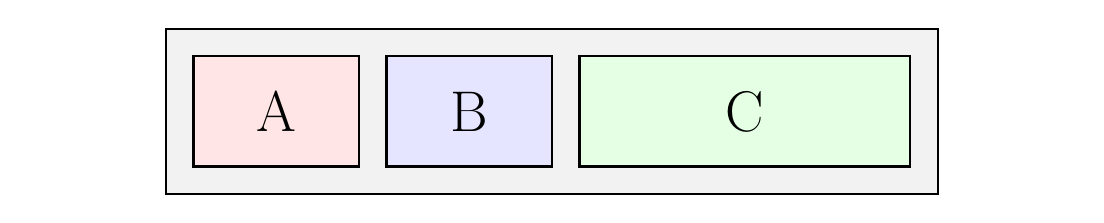
\begin{tikzpicture}[scale=0.07,rotate=0]
	
	%Background
	\draw[draw=white, fill=white] (0,0) rectangle (190,30);
		
	%Frame
	\draw[thick, draw=black, fill=gray!10] (25,0) rectangle (165,30);

	%Segments
	%A
	\draw[thick, draw=black, fill=red!10] (30,5) rectangle (60,25);
	\node at (45,15) {\huge A};

	%B
	\draw[thick, draw=black, fill=blue!10] (65,5) rectangle (95,25);
	\node at (80,15) {\huge B};
	
	%C
	\draw[thick, draw=black, fill=green!10] (100,5) rectangle (160,25);
	\node at (130,15) {\huge C};
	

	
\end{tikzpicture}
\end{document}}
	\caption{Protokoll för överföring av styrkommandon\label{styrdata}}	
\end{figure}

Respektive segment motsvarar följande: 
\begin{itemize}
	\item A (1 byte) - Kommunikations-ID, se tabell \ref{kommunikationstab}.
	\item B (1 byte) - Definierar vilket kommando som skickas, se tabell \ref{tab}.
	\item C (1 byte) - Hastighet om manuellt läge, valfritt i autonomt då det inte tas hänsyn till (tillåtna värden: 0-245).
\end{itemize}

\subsubsection{Kommunikationsprotokoll - kartinformation}
Huvudmodulen skickar för varje ny kartmodul data till datormodulen som ritar upp den nya informationen grafiskt. Varje kartmodul representeras av en position i ett tvådimensionellt fält. För överföring av denna information används protokollet i figur \ref{kartdata}.

\begin{figure}[htbp]
\centering
\noindent\resizebox{.8\linewidth}{!}{
	\documentclass[crop,tikz]{standalone}
\usepackage{tikz}
\usetikzlibrary{calc}
\usetikzlibrary{positioning}
\begin{document}
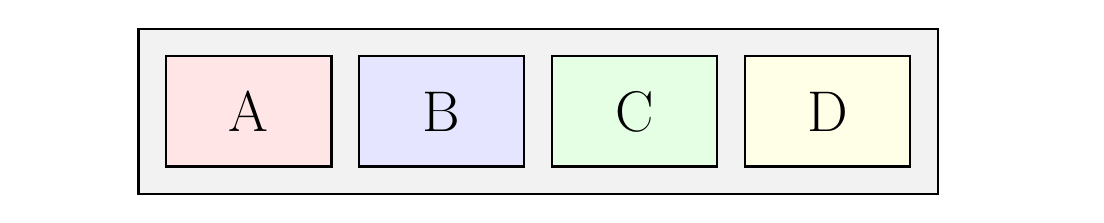
\begin{tikzpicture}[scale=0.07,rotate=0]
		
	%Background
	\draw[draw=white, fill=white] (0,0) rectangle (190,30);	
		
	%Frame
	\draw[thick, draw=black, fill=gray!10] (20,0) rectangle (165,30);

	%Segments
	%A
	\draw[thick, draw=black, fill=red!10] (25,5) rectangle (55,25);
	\node at (40,15) {\huge A};

	%B
	\draw[thick, draw=black, fill=blue!10] (60,5) rectangle (90,25);
	\node at (75,15) {\huge B};
	
	%C
	\draw[thick, draw=black, fill=green!10] (95,5) rectangle (125,25);
	\node at (110,15) {\huge C};
	
	%D
	\draw[thick, draw=black, fill=yellow!10] (130,5) rectangle (160,25);
	\node at (145,15) {\huge D};
	
\end{tikzpicture}
\end{document}}
	\caption{Protokoll för överföring av kartdata \label{kartdata}}	
\end{figure}

Respektive segment motsvarar följande: 
\begin{itemize}
	\item A (1 byte) - Kommunikations-ID, se tabell \ref{kommunikationstab}.
	\item B (1 byte) - x-koordinat (tillåtna värden: 0-30).
	\item C (1 byte) - y-koordinat (tillåtna värden: 0-17).
	\item D (1 byte) - Information om vad som finns i noden, se tabell \ref{tab}.
\end{itemize}

\subsubsection{Kommunikationsprotokoll - sensordata}
Sensordata skickas enligt protokollet i figur \ref{sensordata}.

 \begin{figure}[H]
\centering
\noindent\resizebox{.8\linewidth}{!}{
	\documentclass[crop,tikz]{standalone}
\usepackage{tikz}
\usetikzlibrary{calc}
\usetikzlibrary{positioning}
\begin{document}
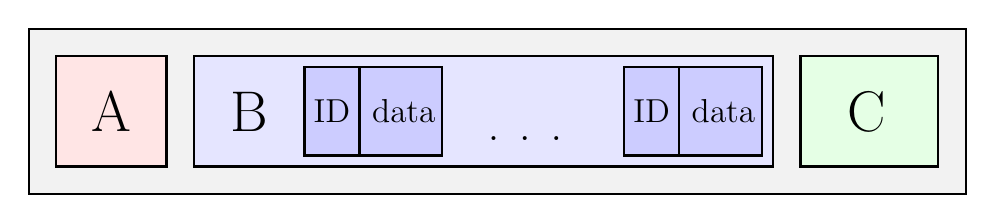
\begin{tikzpicture}[scale=0.07,rotate=0]
		
	%Frame
	\draw[thick, draw=black, fill=gray!10] (0,0) rectangle (170,30);

	%Segments
	%A
	\draw[thick, draw=black, fill=red!10] (5,5) rectangle (25,25);
	\node at (15,15) {\huge A};

	%B
	\draw[thick, draw=black, fill=blue!10] (30,5) rectangle (135,25);
	\node at (40,15) {\huge B};
	
	%B1
	\draw[thick, draw=black, fill=blue!20] (50,7) rectangle (60,23);
	\draw[thick, draw=black, fill=blue!20] (60,7) rectangle (75,23);
	\node at (55,15) {\large ID};
	\node at (68,15) {\large data};
	
	\node at (90,10) {\LARGE . . .};
	
	%Bn
	\draw[thick, draw=black, fill=blue!20] (118,7) rectangle (133,23);
	\draw[thick, draw=black, fill=blue!20] (108,7) rectangle (118,23);
	\node at (113,15) {\large ID};
	\node at (126,15) {\large data};

	%C
	\draw[thick, draw=black, fill=green!10] (140,5) rectangle (165,25);
	\node at (152,15) {\huge C};
	
\end{tikzpicture}
\end{document}}
	\caption{Protokoll för överföring av sensordata\label{sensordata}}	
\end{figure} 

Respektive segment motsvarar följande: 
\begin{itemize}
	\item A - Kommunikations-ID, se tabell \ref{kommunikationstab}.
	\item B - Sensordatapaket
	\begin{itemize}
	\item ID (1 byte) - identifierar sensorn, se tabell \ref{tab}.
	\item Data (1 byte) - sensorns värde (tillåtna värden: 0-245).
	\end{itemize}
\end{itemize}

\subsubsection{Kommunikationsprotokoll - styrinställningar}
Protokollet som används för att skicka styrinställningar, både datormodul $\rightarrow$ huvudmodul och huvudmodul $\rightarrow$ styrmodul finns illustrerat i figur \ref{styrkomm}.

\begin{figure}[htbp]
\centering
\noindent\resizebox{.8\linewidth}{!}{
	\documentclass[crop,tikz]{standalone}
\usepackage{tikz}
\usetikzlibrary{calc}
\usetikzlibrary{positioning}
\begin{document}
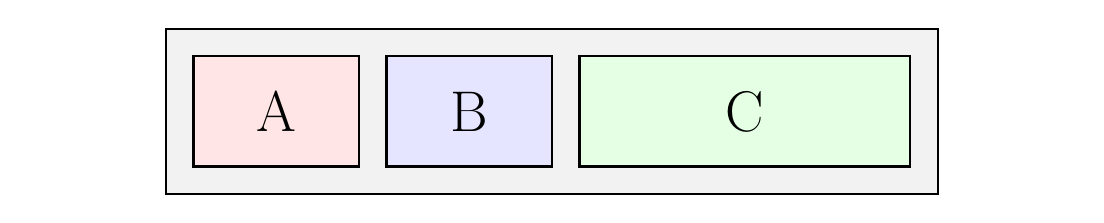
\begin{tikzpicture}[scale=0.07,rotate=0]
	
	%Background
	\draw[draw=white, fill=white] (0,0) rectangle (190,30);
		
	%Frame
	\draw[thick, draw=black, fill=gray!10] (25,0) rectangle (165,30);

	%Segments
	%A
	\draw[thick, draw=black, fill=red!10] (30,5) rectangle (60,25);
	\node at (45,15) {\huge A};

	%B
	\draw[thick, draw=black, fill=blue!10] (65,5) rectangle (95,25);
	\node at (80,15) {\huge B};
	
	%C
	\draw[thick, draw=black, fill=green!10] (100,5) rectangle (160,25);
	\node at (130,15) {\huge C};
	

	
\end{tikzpicture}
\end{document}}
	\caption{Protokoll för överföring av styrinställning \label{styrkomm}}	
\end{figure}

Respektive segment motsvarar följande: 
\begin{itemize}
	\item A (1 byte) - Kommunikations-ID, se tabell \ref{kommunikationstab}.
	\item B (1 byte) - Definierar vilken styrinställning som skickas, se tabell \ref{tab}.
	\item C (1 byte) - 0/1 om av/på, annars flyttal (C float).
\end{itemize}

%\subsubsection{Kommunikationsprotokoll - Positionsinformation}
%Protokollet som används för att skicka positionsinformation finns illustrerat i figur \ref{positionInfo}.

%\begin{figure}[htbp]
%\centering
%\noindent\resizebox{.8\linewidth}{!}{
%	\documentclass[crop,tikz]{standalone}
\usepackage{tikz}
\usetikzlibrary{calc}
\usetikzlibrary{positioning}
\begin{document}
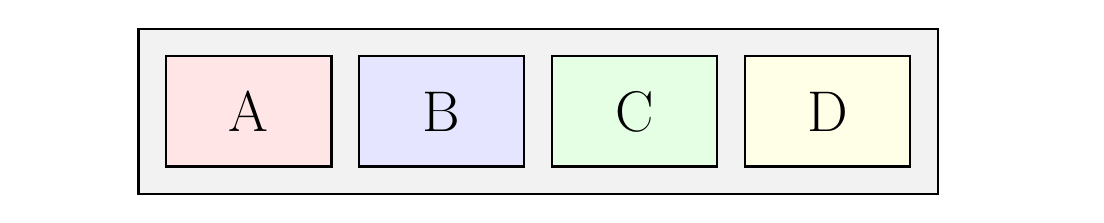
\begin{tikzpicture}[scale=0.07,rotate=0]
		
	%Background
	\draw[draw=white, fill=white] (0,0) rectangle (190,30);	
		
	%Frame
	\draw[thick, draw=black, fill=gray!10] (20,0) rectangle (165,30);

	%Segments
	%A
	\draw[thick, draw=black, fill=red!10] (25,5) rectangle (55,25);
	\node at (40,15) {\huge A};

	%B
	\draw[thick, draw=black, fill=blue!10] (60,5) rectangle (90,25);
	\node at (75,15) {\huge B};
	
	%C
	\draw[thick, draw=black, fill=green!10] (95,5) rectangle (125,25);
	\node at (110,15) {\huge C};
	
	%D
	\draw[thick, draw=black, fill=yellow!10] (130,5) rectangle (160,25);
	\node at (145,15) {\huge D};
	
\end{tikzpicture}
\end{document}}
%	\caption{Protokoll för överföring av positionsinformation \label{positionInfo}}	
%\end{figure}

%Respektive segment motsvarar följande: 
%\begin{itemize}
%	\item A (1 byte) - Kommunikations-ID, se tabell \ref{kommunikationstab}.
%	\item B (1 byte) - x-koordinat (tillåtna värden: 0-30).
%	\item C (1 byte) - y-koordinat (tillåtna värden: 0-17).
%	\item D (1 byte) - riktning.
%\end{itemize}

\pagebreak

\begin{table}[H]
\begin{tabular}{|p{6em}|p{1em}|p{6em}|p{22em}|} \hline

\textbf{Kommando} & \textbf{Id} & \textbf{Info} & \textbf{Kommentar}\\ \hline

252 & 1 & 0/1 & 1 om reglering är på, 0 annars \\ \hline
252 & 2 & Data & Reglerfunktionens P-värde \\ \hline
252 & 3 & Data & Reglerfunktionens D-värde \\ \hline
252 & 9 & 0/1 & 1 om gripklo ska vara öppen, 0 om den ska vara stängd \\ \hline

\end{tabular}

\begin{tabular}{|p{6em}|p{1em}|p{6em}|p{22em}|} \hline
253\text{*}  & 1 & Data & Värde på den främre högra IR-sensorn \\ \hline
 & 2 & Data & Värde på den främre vänstra IR-sensorn \\ \hline
 & 3 & Data & Värde på den bakre högra IR-sensorn \\ \hline
 & 4 & Data & Värde på den bakre vänstra IR-sensorn \\ \hline
 & 5 & Data &  Värde på \verb+Lidar-Lite v2+:s 8 mest signifikanta bitar \\ \hline
 & 6 & Data &  Värde på \verb+Lidar-Lite v2+:s 8 minst signifikanta bitar \\ \hline
 & 7 & Data & Värde på gyrot \\ \hline
 & 8 & Data & Värde för IR-detektorn (1 om målet är upptäckt, 0 annars) \\ \hline
 & 9 & Data & Antal flanker reflexsensorn detekterat sen sist\\ \hline
\end{tabular}

\begin{tabular}{|p{6em}|p{1em}|p{6em}|p{22em}|} \hline

255 & 0 & - & Kommando att stanna \\ \hline
255 & 1 & Data/-\textsuperscript{**}   & Kommando att köra framåt \\ \hline
255 & 2 & - & Kommando att rotera 180 grader\\ \hline
255 & 3 & Data/-\textsuperscript{**}    & Kommando att rotera höger \\ \hline
255 & 4 & Data/-\textsuperscript{**}    & Kommando att rotera vänster \\ \hline
255 & 12 & - & Kommando att köra en halv modul framåt\\ \hline
255 & 13 & - & Kommando att köra en halv modul bakåt \\ \hline
\end{tabular}

\text{*} Gäller för alla efterföljande sensorer då alla värden skickas i samma paket \\*
\text{**} Reagerar på data vid manuellt läge och ignorerar data vid autonomt

\caption{Tabell över informationsflödet} \label{tab}
\end{table}

\pagebreak
\section{Slutsatser}Gruppen känner sig nöjd med uppnått resultat men ser samtidigt utvecklingmöjligheter av produkter inom några områden. 

En av de naturligt följande förbättringarna är att få roboten att kunna navigera i öppna rum, vilket var ett krav av prioritet 2. Nu är roboten begränsad till att operera i en omgivning bestående av ett layrintsystem med vinkelräta svängar. För att utöka dess användningsområde kan även produkten utvecklas så att den kan reglera vid alla typer av svängar, inte bara vinkelräta.

Något som gruppen hade velat utveckla i mån av mer tid är kartläggning i tre dimensioner. Det hade bidragit till en bättre användarupplevelse. I övrigt är gruppen nöjd med robotens funktioner. 

Förbättringspotential finns även i de redan existerande funktionerna. Roboten skulle till exempel kunna göras smartare genom att förbättra avsökningsalgoritmen som i dagsläget inte är helt optimerad. Det skulle göra stor skillnad i en stor och komplicerad bana. 
\pagebreak


\addcontentsline{toc}{section}{Referenser}
\bibliographystyle{ieeetr}
\bibliography{references}

\pagebreak
\appendix
\section{Kopplingsschema}

\section{Kodexempel} \label{App:AppendixA}
Nedan följer kodexempel från de olika modulerna.

\subsection{Huvudmodul}
\lstinputlisting[language=c]{searchPath-v20.h}

\subsection{Sensormodul}
\lstinputlisting[language=c]{mainStable.c}

\subsection{Styrmodul}
\lstinputlisting[language=c,firstline=739, lastline=823]{styrmodulUnstable.c}

\subsection{Datormodul}
\lstinputlisting[language=java,firstline=36, lastline=73]{Log.java}

\lstinputlisting[language=java,firstline=55, lastline=73]{TablePanel.java}

\lstinputlisting[language=java,firstline=13]{SensorData.java}

\pagebreak


\end{flushleft}

\end{document}

